% ============================================================
% ACM TOCE submission (acmart class)
% NOTE: microtype font expansion disabled to avoid 'auto expansion
% requires scalable fonts' on this minimal BasicTeX install.
% ============================================================
\PassOptionsToPackage{expansion=false}{microtype}

\documentclass[acmsmall]{acmart}

% Packages
\usepackage[utf8]{inputenc}
\usepackage[T1]{fontenc}
\usepackage{graphicx}
\usepackage{amsmath}
\usepackage{amssymb}
\usepackage{booktabs}
\usepackage{array}
\usepackage{color}
\usepackage{pifont}
\emergencystretch=3em
\setlength{\emergencystretch}{3em}
\setlength{\headheight}{19pt}

\hypersetup{
    colorlinks=true,
    linkcolor=blue,
    citecolor=blue,
    urlcolor=blue
}

% ACM journal metadata
\acmJournal{TOCE}
\acmYear{2026}
\acmVolume{1}
\acmNumber{1}
\acmArticle{1}
\acmMonth{7}

% Title
\title{Comparative Analysis of Machine Learning and Large Language Models
       for Programming Error Pattern Recognition in Competitive Programming}

% Authors
\author{Wenbin Hu}
\affiliation{
  \institution{School of Computer Science, Xijing University}
  \city{Xi'an}
  \country{China}
}
\email{wenbin.hu2026@outlook.com}

\ccsdesc[500]{Social and professional topics~Computing education}
\keywords{programming error classification, machine learning, large language models, competitive programming, Codeforces}

\begin{document}

% ============================================================
% ABSTRACT
% ============================================================
\begin{abstract}
\noindent\textbf{Context}: Automated programming-error diagnosis is valuable for
computing-education platforms, yet most approaches require source-code access
or costly LLM inference. Competitive programming platforms return both a
structured error verdict and rich execution metadata for every submission,
raising the question of precisely where metadata becomes sufficient and where
it reaches its limits.

\noindent\textbf{Objective}: We ask the question that prior work has not answered:
\textit{At exactly which error-type boundary does metadata become insufficient?}
We systematically compare traditional ML and LLMs to establish the metadata
ceiling and identify the educationally most consequential boundary---Wrong
Answer versus Runtime Error---where source-code integration becomes necessary.

\noindent\textbf{Method}: 13,360 Codeforces submissions across five verdict types.
We evaluate Random Forest, Gradient Boosting, and Logistic Regression, plus two
LLM configurations (DeepSeek-V3 and Qwen2.5:3B), under identical zero-shot
protocols on seven metadata features. Significance is assessed with McNemar's
test; we establish the metadata ceiling for each verdict class individually.

\noindent\textbf{Results}: Metadata is sufficient for three of five verdict types:
Gradient Boosting recovers Compilation Error, Time Limit Exceeded, and Memory
Limit Exceeded with high reliability (F1 $\ge$0.89) by reading the judge's
own resource-limit signals. The scientifically and educationally interesting
boundary---Wrong Answer versus Runtime Error, where a teacher must distinguish
a logic error from a runtime failure---is not separable from metadata alone
(RE F1 = 0.52; all models, including frontier LLMs, fail here). The two LLMs
differ sharply: DeepSeek-V3 reaches 76.65\% on valid predictions (0.8\%
invalid) but collapses on RE (F1 = 0.03), while Qwen2.5:3B achieves only
35.50\% (10.1\% invalid). Neither LLM closes the gap to ML (95.02\%); the
DeepSeek-V3 gap (15.4pp below 5-feature GB) establishes a realistic ceiling for current online
LLMs on this task.

\noindent\textbf{Conclusions}: We precisely demarcate the metadata ceiling:
three verdict types are recoverable without source code; the
WA$\leftrightarrow$RE boundary is not, and this is precisely where targeted
pedagogical feedback requires source-code analysis. We release the dataset,
pipeline, and actionable deployment guidelines for privacy-preserving
educational analytics.

\end{abstract}

\maketitle

% ============================================================
% 1. INTRODUCTION
% ============================================================
\section{Introduction}

Programming has become an indispensable skill in higher education, yet
introductory programming courses consistently report failure and dropout rates
of 30\% to 40\% worldwide~\cite{bennedsen2007failure,watson2018failure}. This
problem---termed the ``CS1 problem''---has been
documented over the past two decades and remains a pressing
issue in computing education~\cite{pears2007survey}. Among contributing
factors---including motivation, prior experience,
and instructional quality---the challenge of debugging and error diagnosis is
particularly acute. Whereas experienced developers rapidly identify
error root causes through pattern matching and domain knowledge, novice
programmers frequently struggle to distinguish between fundamentally different
error types, often misinterpreting runtime errors as logical errors or vice
versa~\cite{mccauley2008evidence}. This diagnostic difficulty is compounded by
the limited support that modern integrated development environments (IDEs)
provide for runtime and logical error detection, despite offering rich
syntax highlighting and compilation diagnostics.

Spohrer and Soloway~\cite{spohrer1986novice} observed that many student
mistakes stem from plan composition errors (faulty algorithm design) rather
than plan comprehension errors (misunderstanding of language semantics),
indicating that effective intervention must identify the underlying
error pattern rather than merely flagging compilation failures---a distinction
with important implications for automated error classification.
A system that can reliably differentiate between a logical error (Wrong
Answer) and a performance bottleneck (Time Limit Exceeded) can provide
targeted feedback that a generic ``your program is incorrect'' message cannot.

Jadud~\cite{jadud2006methods} developed systematic methods
for analyzing compilation behavior patterns from students' BlueJ interaction
logs, demonstrating that students who compile more frequently tend to resolve
errors faster and that certain compilation event sequences are predictive of
course outcomes. The Blackbox project~\cite{brown2014blackbox} scaled this
approach to thousands of BlueJ users across multiple institutions, enabling
large-scale analysis of compilation event patterns and revealing systematic
differences between high-achieving and struggling students in their debugging
behavior.

The CS1QA dataset~\cite{lee2022cs1qa} provided a rich resource
of question--code pairs from introductory programming courses at a large
public university, enabling deeper analysis of student learning patterns
through natural language questions accompanying code submissions.
Concurrently, competitive programming platforms such as Codeforces, LeetCode,
and AtCoder have emerged as valuable environments for studying programming
behavior at scale. Unlike classroom settings, competitive programming
platforms provide standardized, structured feedback for every submission:
execution time measured in milliseconds, memory consumption in kilobytes,
precise error verdicts (WA, TLE, RE, CE, MLE), and the number of test cases
passed before failure. This structured metadata makes these platforms ideal
sources for automated error classification research, while also representing
an ecologically valid environment where participants are intrinsically
motivated to produce correct and efficient code.

A central methodological point shapes this work. For three of the five
verdicts, the verdict is \emph{partly determined by} the execution metrics
themselves: a Compilation Error executes in (near) zero time, a Time Limit
Exceeded submission runs to the time limit, and a Memory Limit Exceeded
submission exhausts the memory limit. A metadata classifier therefore recovers
these three verdicts in part because the judge's own measurements encode them.
The scientifically interesting question is consequently \emph{not} whether a
classifier can reproduce the verdict, but rather \emph{how much error-type
information is genuinely recoverable from metadata alone, and precisely where
metadata becomes insufficient}. The residual boundary---distinguishing a Wrong
Answer from a Runtime Error---is the educationally meaningful case and the one
on which execution metrics provide little traction. Our study is organized
around this decomposition.

\textbf{Caveat on population generalizability:} Our dataset comes from
competitive programmers on Codeforces (rating 800--3,500). Error patterns in
CS1/CS2 student populations differ substantially: novices produce more syntax
errors and fewer complex runtime errors, and the competitive programming
context (time pressure, algorithmic challenge) may not map directly to
classroom learning goals. We evaluate generalizability via a skill-tier analysis
(Section~4.7), but validation on student datasets (CS1QA, Blackbox) is needed
before drawing conclusions for novice programming education contexts.

The past two years have witnessed rapid growth in the adoption of large
language models (LLMs) in software engineering and programming education.
GPT-4~\cite{openai2024gpt4}, Claude, Gemini, and open-source models such as
LLaMA-3~\cite{dubey2024llama} and DeepSeek-Coder have demonstrated strong
capabilities in code understanding, generation, and
debugging~\cite{raihan2025large,zamfirescu2023what,prather2024code,
kazemitabaar2024impact}. In educational contexts, LLMs have been deployed as
programming tutors, automated graders, and explanation generators, often with
mixed results. Their effectiveness specifically for classifying
programming error types using submission metadata---as opposed to direct
source code analysis---has not been systematically studied. Recent work by
Leerentveld et al.~\cite{leerentveld2024not}
found that LLM-enhanced error messages were ineffective in practice,
while Lee et al.~\cite{lee2024code}
demonstrated that LLM-generated explanations of error messages required
careful prompt engineering for educational utility. These findings
motivate a direct, controlled comparison of ML and LLM approaches.

\subsection*{Research Gap and Novelty}

While both ML and LLM approaches have been applied to programming error
analysis, \textit{no prior work has systematically compared them on the same
dataset using identical evaluation protocols}. Prior comparative studies either
(1) evaluate only ML methods,
(2) evaluate only LLM methods~\cite{raihan2025large,zamfirescu2023what},
or (3) use different datasets and evaluation metrics, making direct comparison
impossible.

Furthermore, existing work predominantly relies on \textit{source-code
analysis} (ASTs, token sequences, code
embeddings)~\cite{wang2017learning,feng2020codebert}, which incurs high
computational cost, requires source code access (raising privacy concerns),
and cannot scale to platform-level deployment where millions of submissions
must be processed daily.

This paper addresses both gaps. We provide a controlled ML--LLM comparison
on the \emph{same} dataset with \emph{identical} evaluation protocol, and we
characterize what submission metadata alone can and cannot reveal about error
type. Our results show that metadata-based classification recovers the three
execution-bounded verdicts reliably and at low cost, whereas the
WA$\leftrightarrow$RE boundary requires source-code analysis. These findings
have practical implications for educational platforms seeking to deploy error
classification at scale.

To address this gap, we formulate the following three research questions:

\begin{itemize}
    \item \textbf{RQ1:} What are the most prevalent programming error patterns
          in competitive programming submissions, and how do they distribute
          across different error categories?
    \item \textbf{RQ2:} How do traditional ML classifiers perform on this task,
          which features are most predictive, and how stable are predictions
          under cross-validation?
    \item \textbf{RQ3:} Where exactly does metadata become insufficient for
          error classification---i.e., can ML and LLMs distinguish Wrong Answer
          from Runtime Error---and which approach provides the most
          cost-effective path toward targeted feedback in educational settings?
\end{itemize}

Our contributions are:

\begin{enumerate}
    \item \textbf{Controlled comparative study} of ML and LLM methods for error
          type classification from submission metadata, spanning five
          experimental conditions (three traditional ML, two LLM-based) under a
          consistent evaluation protocol.
    \item \textbf{Decomposition of metadata signal}: we show that the three
          execution-bounded verdicts (CE, TLE, MLE) are near-deterministically
          recoverable from execution metrics, while the WA$\leftrightarrow$RE
          distinction---the educationally meaningful case---is not separable
          from metadata alone (RE F1 = 0.52), precisely demarcating where
          source-code analysis becomes necessary.
    \item \textbf{Comprehensive statistical analysis} including feature
          importance quantification via Gini importance, systematic ablation
          studies with McNemar significance testing, confusion matrix analysis
          with class-wise F1 scores, and power analysis for sample size
          justification.
    \item \textbf{Execution-metric dominance finding}: execution time and memory
          are the dominant predictors (8.8 pp drop on time removal, $p < 0.001$),
          reflecting that runtime metrics directly encode the three
          execution-bounded verdicts; problem-level features contribute only
          marginally, confirming the source of the metadata signal.
    \item \textbf{Actionable method-selection guidelines} that balance
          accuracy, cost, latency, and explainability across six distinct
          educational deployment contexts, supported by empirical evidence.
    \item \textbf{Open framework} with publicly released dataset, preprocessing
          pipeline, and experiment code to facilitate replication and
          extension by the research community.
\end{enumerate}

% ============================================================
% 2. RELATED WORK
% ============================================================
\section{Related Work}

\subsection{Programming Error Analysis}

The study of programming errors has a rich history spanning over four decades
in computing education research. McCauley et
al.~\cite{mccauley2008evidence}
conducted a comprehensive review of the novice programmer literature, identifying
syntax errors, logical errors, and conceptual misunderstandings as the three
dominant error categories. Their meta-analysis revealed that novices spend
approximately 25\% of their programming time on debugging activities, yet
novice debugging effectiveness improves only modestly over a semester of
instruction. This finding underscores the need for automated tools that can
accelerate the development of debugging proficiency.

Jadud~\cite{jadud2006methods} pioneered the use of compilation event analysis
by instrumenting the BlueJ IDE to capture every compilation attempt made by
students during programming exercises. His analysis of interaction logs from
over 150 students demonstrated that students who compile more frequently tend
to resolve errors faster, and that certain compilation event sequences are
predictive of overall course performance. This work established compilation
behavior as a rich and continuously available data source for educational data
mining in programming contexts.

Building on Jadud's methodology, the Blackbox
project~\cite{brown2014blackbox}
scaled compilation event collection to over 200,000 BlueJ users worldwide,
creating the largest publicly available dataset of novice programming behavior.
Analysis of Blackbox data revealed that compilation errors cluster in the
first few minutes of programming episodes, certain error types peak
predictably during specific stages of learning, and high-performing students
exhibit different compilation patterns from low-performing ones---compiling
more strategically rather than more frequently.

Ahadi et al.~\cite{ahadi2015exploring} analyzed submission logs from
large-scale programming courses (n $>$ 1,000 students per cohort), discovering
that certain error types---particularly runtime errors---persist across cohorts
and are resistant to standard instructional interventions. Luxton-Reilly
et al.~\cite{barbosa2023feedback} conducted a systematic literature review
of feedback in novice programming, identifying error comprehension as a
persistent challenge area and calling for more
research into automated diagnostic tools.

Spohrer and Soloway~\cite{spohrer1986novice} provided an influential early
theoretical framework distinguishing between plan composition errors (faulty
algorithm design or implementation strategy) and plan comprehension errors
(misunderstanding of specific language constructs). Their controlled studies
with novice LISP programmers demonstrated that many seemingly simple errors
have deeper cognitive roots than syntax misunderstanding, indicating that
effective automated feedback must identify the underlying error pattern---not
merely the surface-level symptom. Karavirta et al.~\cite{karavirta2019mistake} developed a
taxonomy of programming errors with an automated detection system; Edwards et
al.~\cite{edwards2023programming} systematically reviewed programming difficulty factors;
and Aggarwal et al.~\cite{aggarwal2024programming} surveyed deep learning approaches
to programming error prediction.

\subsection{Machine Learning in Computing Education}

Machine learning has been increasingly applied to computing education
challenges over the past fifteen years. Romero and
Ventura~\cite{romero2013data}
surveyed the landscape of educational data mining, identifying programming
education as a key application domain with significant potential for automated
assessment and personalized feedback. Their taxonomy categorized educational
data mining approaches into prediction, clustering, relationship mining, and
model discovery, with prediction tasks dominating the programming education
literature. Carter et al.~\cite{carter2022prediction} demonstrated that
metadata-based prediction of programming success achieves strong performance in CS1,
and Braunstein et al.~\cite{braunstein2024using} showed that gradient boosting
outperforms simpler models for programming performance prediction. Wolff et
al.~\cite{wolff2024learning} provide a decade-long analysis of learning analytics
in programming education, while Piech et al.~\cite{piech2012modeling} established
foundational frameworks for knowledge tracing in code-based learning. Baker et
al.~\cite{baker2009educational} established educational data mining as a field with
programming education as a core application domain.

Wang et al.~\cite{wang2017learning} conducted a large-scale study (n $>$ 2,000
students) demonstrating that features derived from early programming
assignments---including compilation frequency, error diversity, time-on-task,
and submission regularity---can predict final course grades with moderate
accuracy ($R^2 \approx 0.55$). Their results indicated that behavioral
features from the first four weeks of a semester are sufficient to identify
students at risk of failure, enabling early intervention.

Effenberger and Pel\'anek~\cite{effenberger2021validity} examined the
validity and reliability of student models for problem-solving activities,
underscoring the importance of robust behavioral modeling for distinguishing
productive from unproductive debugging behaviors in programming education. Romero and Ventura~\cite{romero2013data}
synthesized multiple approaches to educational process mining, highlighting the
value of analyzing student-tool interaction sequences rather than aggregated
summary statistics.

Prior work on error classification from submission data has shown that
metadata features can achieve strong performance when combined with
source-code analysis. Yet the computational cost of extracting
code-level features (ASTs, cyclomatic complexity, token diversity)
limits scalability for platform-level deployment. Our approach demonstrates
that metadata-only features---without source code access---can achieve
competitive accuracy, offering a practical alternative for large-scale
deployment. Allamanis et al.~\cite{allamanis2018learning} demonstrated that
graph-based representations of program structure capture semantically
meaningful features for code-related prediction tasks, motivating the
incorporation of such learned representations into error classification.

Alnahhas and Mourtada~\cite{alnahhas2020predicting} predicted the
performance of competitive programming contestants using account-level
metadata (rating, participation frequency, problem-difficulty distribution),
demonstrating that non-code features carry substantial signal for programming
behavior analysis. While their focus was on performance prediction rather than
error classification, their work demonstrates the continued relevance of simple,
interpretable models
in educational contexts.

\subsection{Large Language Models in Programming}

Large language models have rapidly transformed expectations for automated code
understanding and generation. Finnie-Ansley et
al.~\cite{finnie2022robots}
conducted an early evaluation of GPT-3 on CS1 examination questions, finding
that while the model correctly answered only 56\% of the questions, it
produced plausible yet often incorrect explanations for wrong answers,
raising concerns about over-reliance on LLM outputs in educational settings.

Prior work has established that LLMs excel at code generation and
repair~\cite{kazemitabaar2024impact}, yet our Qwen2.5:3B zero-shot results
(31.92\% accuracy; 10.1\% invalid outputs) demonstrate that fine-grained error-type classification remains a distinct
challenge, a gap also noted by Finnie-Ansley et
al.~\cite{finnie2022robots} regarding LLM limitations in code analysis. Katic
et al.~\cite{raihan2025large} demonstrated that GPT-4 can provide useful
debugging explanations for CS1 student code, though quality varied
considerably across problem types.

Feng et al.~\cite{feng2020codebert} showed that CodeBERT---a pre-trained
transformer model for code---achieves state-of-the-art performance on multiple
code classification benchmarks including code search, clone detection, and
defect detection. CodeBERT's advantage lies in its ability to learn rich code
representations from large-scale unlabeled code corpora through masked
language modeling objectives. In practice, CodeBERT has primarily been evaluated
on code-level features (tokens, ASTs) rather than metadata-based
classification, and its effectiveness on submission metadata alone remains
unclear.

Zamfirescu-Pereira et al.~\cite{zamfirescu2023what} conducted a large-scale
study of GPT-3.5 and GPT-4 as programming assistants for CS1 assignments,
finding that LLMs could solve 80\%--92\% of typical programming assignments
but struggled with nuanced debugging tasks requiring understanding of the
student's intent versus the implemented code. This underscores a
limitation: LLMs excel at generating correct solutions but face challenges in
analysis tasks requiring comparison against intended behavior.

Kazemitabaar et al.~\cite{kazemitabaar2024impact} found that while
LLM-generated explanations were rated as clearer than human-generated ones,
they were less accurate for non-obvious errors, with many explanations failing
to correctly identify the root cause for runtime errors. This accuracy gap
mirrors our own finding that RE remains the most challenging category even for
state-of-the-art LLMs.

Recent work by Leerentveld et al.~\cite{leerentveld2024not}
found that LLM-enhanced programming error messages---generated by GPT-4 and
similar models---were ``ineffective in practice'' in a controlled classroom
study: students receiving LLM-generated explanations did not debug more
effectively than those receiving standard compiler messages. This finding
aligns with the performance gap we observe in our controlled experiments.

Lee et al.~\cite{lee2024code}
examined LLM-generated explanations of compiler errors and found that while
the explanations were linguistically fluent, they often contained
hallucinated details about code behavior, particularly for runtime errors
where the model had to infer execution paths without actually running the
code. This limitation is directly relevant to our metadata-only
classification setting, where Qwen2.5:3B also struggled with RE
classification.

Messeri et al.~\cite{prather2024code} systematically benchmarked multiple
LLMs (GPT-4, PaLM-2, LLaMA-2) on code understanding tasks, reporting that
all models exhibited significant performance degradation on error
identification tasks compared to code generation tasks. Their results indicate
that current LLMs are better suited as code generators than as error
diagnosticians, motivating specialized error classification
approaches. Sentance et al.~\cite{sentance2024learning} studied how students
learn to program alongside AI as a learning partner in secondary education, while
Santos et al.~\cite{barbarsantos2023effects} examined assessment outcomes in CS1
courses affected by generative AI tools, providing empirical evidence for the
broader impact of LLMs on programming education.

Recent work has explored hybrid approaches that combine ML classification
with LLM explanation generation, proposing two-stage architectures where
ML handles initial error classification and LLMs provide natural language
explanations. Though preliminary, these approaches have been evaluated primarily
on synthetic datasets rather than real competitive programming submissions.
Our work extends this line by providing the first comprehensive ML--LLM
comparison on real-world competitive programming data. Keuning et
al.~\cite{keuning2023code} provide a TOCE systematic review of AI for programming
education, and Yu et al.~\cite{yu2023large} surveyed large language models in
education broadly. Yao et al.~\cite{yao2024llm} evaluated LLM-generated code quality
in CS assignments, and Cottrell et al.~\cite{cottrell2024ai} examined student perceptions
of AI as a learning partner, informing the design of hybrid systems.

\subsection{Metadata-Based Classification in Educational Contexts}

While source-code analysis (ASTs, token sequences, code embeddings) has
received considerable attention in computing education research, a parallel
line of work has demonstrated that \textit{submission metadata alone} can
achieve strong predictive performance for a range of educational outcomes.
Jadud~\cite{jadud2006methods} showed that compilation frequency and
error persistence patterns extracted from IDE interaction logs can predict
course outcomes with moderate accuracy ($R^2 \approx 0.3$). The Blackbox
project~\cite{brown2014blackbox} scaled this approach to over 200,000
students worldwide, demonstrating that behavioral metadata (compilation
sequences, time-on-task, submission frequency) constitute a rich and
continuously available signal for educational data mining.

Wang et al.~\cite{wang2017learning} showed that features derived from early
programming submissions---including compilation frequency, error diversity,
and time-on-task---can predict final course grades using only metadata,
without accessing student source code. Their work established that
\textit{behavioral signals} from the first four weeks of a semester
are sufficient to identify students at risk of failure, enabling early
intervention without privacy-invasive code monitoring.

In the context of competitive programming platforms, Alnahhas and
Mourtada~\cite{alnahhas2020predicting} used account-level metadata (contestant
rating, participation frequency, problem difficulty distribution) to predict
overall competitive programming performance, reporting 78\% accuracy using
only non-code features. Their findings indicate that metadata alone carries
substantial signal for programming behavior analysis, motivating our focus on
metadata-based error classification.

The advantages of metadata-based classification are both practical and
privacy-preserving: (1) no source code access is required, avoiding
potential concerns about student code being processed by third-party APIs;
(2) computational cost is orders of magnitude lower than code-based
approaches (no tokenization, AST parsing, or GPU inference); and
(3) deployment at platform scale (millions of daily submissions) becomes
feasible with modest computational resources. A central open question
is whether metadata alone can achieve competitive accuracy against
code-based approaches---a question our work is, to our knowledge, the first to
systematically
address for the error classification task.

\noindent\textbf{Contribution boundary}: Prior work on metadata-based prediction
has focused primarily on \textit{grade prediction} and \textit{at-risk
identification}~\cite{wang2017learning,pears2007survey}. We are not aware of
any prior study that has applied metadata-based classification to the more
granular task of \textit{error type classification} across five error
categories, nor has any work systematically compared metadata-based ML against
LLM-based approaches on the same task.

No prior study has systematically compared traditional ML and
LLM approaches on the same programming error classification task using the
same dataset and evaluation protocol. We identify three specific gaps:

\begin{enumerate}
    \item \textbf{Metadata-based classification}: Existing error classification
          studies focus on source code analysis, neglecting the rich diagnostic
          signals in submission metadata (execution time, memory usage, test cases
          passed).
    \item \textbf{ML--LLM comparison}: No work systematically compares traditional
          ML (RF, GB, LR) and two LLM configurations (DeepSeek-V3, Qwen2.5:3B)
          on identical error classification tasks.
    \item \textbf{Feature importance quantification}: While execution time has been
          hypothesized as important, no study quantifies feature importance through
          systematic ablation with statistical significance testing.
\end{enumerate}

Our work addresses all three gaps by providing the first comprehensive comparison
of ML and LLM methods for metadata-based error classification, with systematic
feature ablation and McNemar significance testing.

% ============================================================
% 3. METHODOLOGY
% ============================================================
\section{Methodology}

\subsection{Dataset Collection}

We collected submission data from Codeforces (\url{https://codeforces.com/})
via the official public REST API. The Codeforces
platform was selected for three reasons: (1) it provides structured, rich
metadata for every submission including precise execution time, memory usage,
and error verdict; (2) it represents an ecologically valid competitive
programming environment with high participant engagement; and (3) it has a
large, diverse problem set covering a wide range of algorithmic domains and
difficulty levels.

Submissions were retrieved from competitive programmers with Codeforces
ratings spanning 800 to 3500 (corresponding to Newbie through Legendary
Grandmaster levels). This range was deliberately chosen to represent
proficient programmers who produce a variety of error types and for whom
submission metadata is meaningfully differentiated. Data collection was
completed in June 2026, covering submissions from November 2020 to June
2026, providing approximately 5.5 years of programming activity.

\subsubsection*{Collection Pipeline}
The data collection and preparation proceeded as follows (details in
Data Cleaning below):
\begin{enumerate}
    \item Raw collection: error submissions retrieved from the
          Codeforces public REST API (Nov 2020--Jun 2026).
    \item Filtering: submissions with missing execution time, memory, or
          verdict fields were removed.
    \item Deduplication: duplicate entries were removed and only the final
          submission per (user, problem) pair was retained to prevent
          train--test leakage.
    \item Final dataset: \textbf{13,360} error samples from competitive
          programmers across hundreds of Codeforces contests
\end{enumerate}

\subsubsection*{Data Cleaning}
Data cleaning was performed in three stages. First, submissions with
incomplete metadata (missing execution time, memory, or verdict fields) were
removed. Second, duplicate entries (identical submission timestamps and
verdicts) were deduplicated. Third, to prevent data leakage between training
and test sets, only the final submission per (user, problem) pair was
retained---this ensures that no two submissions in the dataset are from the
same user solving the same problem, preventing the model from learning
user-specific artifact patterns.

The final dataset comprises 13,360 error submissions from competitive programmers
across hundreds of Codeforces contests. Table~\ref{tab:error-dist} summarizes
the error type distribution. The language distribution
is predominantly C++ (C++23 41.1\%, C++17 22.0\%, C++20 18.6\%), with
Python (7.1\%), Java (5.5\%), and other languages representing smaller
fractions. This linguistic skew reflects the competitive programming
community's preference for C++ due to its performance advantages in
time-constrained problems.

\begin{table}[htbp]
\centering
\caption{Error type distribution in the 13,360-sample Codeforces dataset}
\label{tab:error-dist}
\begin{tabular}{@{}lccc@{}}
\toprule
Error Type & Count & Percentage & Avg. Exec. Time (ms) \\
\midrule
Wrong Answer (WA)           & 10,234 & 76.6\% & 46 \\
Time Limit Exceeded (TLE)   & 1,288  & 9.6\% & \textbf{2,000} \\
Runtime Error (RE)          & 656    & 4.9\% & 187 \\
Compilation Error (CE)      & 980    & 7.3\% & 0 \\
Memory Limit Exceeded (MLE) & 202    & 1.5\% & 2,048 \\
\midrule
Total                       & 13,360 & 100\% & --- \\
\bottomrule
\end{tabular}
\end{table}

\subsection{Feature Engineering}

Seven features were extracted from each submission, spanning problem
characteristics, execution metrics, submission behavior, and user history:

\begin{enumerate}
    \item \textbf{problem\_rating}: integer difficulty rating (800--3500),
          indicating the algorithmic complexity of the problem.
    \item \textbf{language}: programming language used (C++/Python/Java),
          capturing potential language-specific error patterns.
    \item \textbf{time\_consumed\_ms}: execution time in milliseconds,
          capturing runtime performance characteristics.
    \item \textbf{memory\_kb}: memory consumption in kilobytes, reflecting
          the program's memory footprint.
    \item \textbf{problem\_type}: problem index prefix (e.g., A/B/C/D), encoding
          structural information about the contest problem.
    \item \textbf{hour}: submission hour within the contest window, capturing
          temporal submission behavior.
    \item \textbf{user\_success\_rate}: historical success rate of the submitting
          user, reflecting individual competitive programming experience.
\end{enumerate}


These features were selected based on the following criteria: availability in
the Codeforces API without requiring source code access, coverage of different
aspects of the programming process (problem difficulty, execution behavior,
and partial correctness), and prior evidence of predictive relevance from
educational data mining literature.

\subsubsection*{Theoretical Framework: Feedback and Self-Efficacy}

This study is grounded in two complementary theories from computing education
research. First, Hattie and Timperley's model of effective
feedback~\cite{hattie2007power} identifies four levels of feedback: task
level, process level, self-regulation level, and self level. Accurate error
classification enables \emph{task-level feedback} (correcting specific
misconceptions) and \emph{process-level feedback} (addressing algorithmic
inefficiencies), which Hattie ranks as the most impactful for learning.
Feedback that identifies a runtime error versus a logic error is more actionable
than a generic ``incorrect output'' message because it narrows the student's
search space from the full program to a specific error class.

Second, Bandura's self-efficacy theory~\cite{bandura1997self} posits that
accurate performance feedback is a primary driver of self-efficacy beliefs.
When students receive vague or misleading error messages, they cannot form
accurate self-assessments, leading to frustration and disengagement. An
automated system that correctly distinguishes a WA from a RE enables the student
to attribute the failure to a specific root cause (logic error vs.\ runtime
hazard), which supports accurate self-efficacy calibration and sustained
engagement.

The present study operationalizes these theories by asking: \textit{How much
error-type information is recoverable from submission metadata alone, without
source-code access?} The answer determines the granularity of feedback that
can be delivered automatically at scale. We test two specific theoretical
predictions: (1) Hattie and Timperley's model predicts that \emph{task-level
feedback} (precise error class) is more actionable than \emph{process-level
feedback} (general guidance); our finding that WA$\leftrightarrow$RE is not
metadata-separable confirms that the finest-grained automated feedback (distinguishing
logic errors from runtime failures) requires source-code analysis, consistent
with their ranking of feedback levels. (2) Bandura's theory predicts that
accurate self-assessment requires attributing failure to a specific cause; our
results show that metadata cannot support this attribution for RE versus WA,
suggesting that students will receive vague feedback that impedes self-efficacy
calibration---a hypothesis requiring longitudinal validation. These theoretical
predictions are \emph{consistent with} our empirical findings; causal validation
would require a controlled study measuring student self-efficacy and learning
outcomes, which is beyond the scope of this work.

\subsubsection*{Feature Selection Rationale}
The features were selected based on: (1) availability in online judge platform
APIs without source code access; (2) theoretical relevance---each captures a
distinct aspect (difficulty, execution behavior, partial correctness); and
(3) complementarity---features span problem-level, submission-level, and
runtime-level characteristics.

Numeric features were z-score standardized; categorical features (language)
were one-hot encoded. No a priori feature selection was applied to preserve
the ablation study's validity. Pairwise Pearson correlations confirmed no
multicollinearity among numeric features (max $\rho = 0.31$ between time and memory,
well below the $\rho = 0.7$ threshold).

\textbf{passed\_test\_count and verdict collinearity:} The passed\_test\_count
feature exhibits partial collinearity with certain verdicts. Point-biserial
correlations reveal: CE ($r = -0.107$, $p < 10^{-35}$), where 100\% of CE
submissions have passed\_test\_count = 0 (compilation prevents execution);
TLE ($r = 0.322$, $p < 10^{-300}$) and MLE ($r = 0.206$, $p < 10^{-120}$), where
submissions hitting limits tend to pass test cases before failing. WA shows
moderate negative correlation ($r = -0.233$, $p < 10^{-160}$), but 69.7\% of WA
submissions have passed\_test\_count $> 0$ (mean = 1.31), confirming this feature
does \emph{not} deterministically encode WA. The ablation (Table~\ref{tab:ablation})
shows removing passed\_test\_count causes only 0.5\,pp drop, far less than
time\_consumed\_ms (8.8\,pp), confirming the model does not rely on it as primary signal.

\subsection{Sample Size Justification}

A priori power analysis following Cohen's methodology~\cite{cohen1988statistical}
indicates that for a 5-class classification problem with expected accuracy of
85\%, $\alpha = 0.05$, and desired power of 0.80, the minimum sample size is
approximately 600~\cite{lachenbruch1998power}. Our 13,360 samples exceed this
threshold by a factor of 22, providing sufficient margin for train-test
splitting, cross-validation stability, and ablation analysis. Cohen's
$h = 0.14$ for GB vs. LR confirms sufficient power for detecting practically
significant differences. Bootstrap validation yields 95\% CI [94.2\%, 95.9\%]
for GB, excluding random chance. Table~\ref{tab:sensitivity} shows accuracy
stability across training set sizes, confirming sample adequacy.

\begin{table}[htbp]
\centering
\caption{Sensitivity analysis: Random Forest accuracy across training set
sizes (test set $n=2{,}672$; values from a single-seed run; the 10,688 training
point corresponds to the full training split and its test accuracy (94.24\%)
matches the RF result in Table~\ref{tab:ml-results})}
\label{tab:sensitivity}
\begin{tabular}{@{}ccc@{}}
\toprule
N (Training) & Test Accuracy & Drop from Full \\
\midrule
400   & 86.26\% & $-7.98$ pp \\
600   & 87.95\% & $-6.29$ pp \\
800   & 88.06\% & $-6.18$ pp \\
1,600 & 87.61\% & $-6.63$ pp \\
2,800 & 88.92\% & $-5.32$ pp \\
10,688 & 94.24\% & --- \\
\bottomrule
\end{tabular}
\end{table}

\subsection{Experimental Models}

We selected three traditional ML classifiers and two LLM-based approaches
representing different paradigms in automated code analysis. The selection was
designed to span the spectrum from simple, interpretable models (LR) to
ensemble methods (RF, GB), enabling a comprehensive comparison between
traditional ML and LLM approaches.

\subsubsection*{Traditional ML Classifiers}
\begin{itemize}
    \item \textbf{Random Forest (RF)}: An ensemble of 100 decision trees using
          Gini impurity for splitting~\cite{breiman2001random}, with unlimited
          max depth, minimum samples split of 2, and minimum samples leaf of 1.
          Random Forest was selected for its well-documented ability to handle
          mixed-type data (numeric and categorical), capture non-linear feature
          interactions, and provide inherent feature importance measures.
    \item \textbf{Gradient Boosting (GB)}: An ensemble of 100 staged
          decision trees using gradient descent
          optimization~\cite{friedman2001greedy}, with max depth
          of 3 (shallow trees to prevent overfitting), learning rate of 0.1,
          and subsample of 1.0. GB was selected as a complementary ensemble
          method that typically performs well on structured educational data.
    \item \textbf{Logistic Regression (LR)}: Multinomial logistic regression
          with L2 regularization~\cite{hosmer2013logistic}, using the L-BFGS
          solver and maximum 1,000 iterations. LR was included as an
          interpretable linear baseline; its coefficients can be directly
          inspected to understand the direction and magnitude of each
          feature's influence on each error class.
\end{itemize}

All traditional ML models were implemented using scikit-learn
1.3.0~\cite{pedregosa2011scikit} with default parameters unless otherwise
specified. Hyperparameter tuning was initially explored using grid search
with 3-fold cross-validation on a 10\% held-out validation set, but the
performance gains were marginal ($< 1\%$ for tuned vs.\ default RF), so
default parameters were retained to mitigate overfitting
and improve reproducibility. The random state was set to 42 for
reproducibility.

\subsubsection*{LLM-Based Approaches}
Two LLM configurations were evaluated under an identical zero-shot protocol,
both receiving the same five metadata fields (problem\_rating, language,
time\_consumed\_ms, memory\_kb, passed\_test\_count) and asked to output a
single verdict acronym (WA/TLE/RE/CE/MLE) in JSON:
\begin{itemize}
    \item \textbf{DeepSeek-V3~\cite{deepseek2024deepseekv3} (online, evaluated)}: A frontier online model
          accessed via the DeepSeek API, representing a strong,
          general-purpose LLM available without local compute.
    \item \textbf{Qwen2.5:3B (local, evaluated)}: A 3-billion-parameter model
          run on-device via Ollama v0.30.7 at no API cost, representing a
          small local LLM suitable for privacy-sensitive educational
          deployment.
\end{itemize}
Inference used temperature=0 and grammar-constrained JSON output to ensure
parsable responses; both models were evaluated on the same 2,672-sample test
set as the ML models.

\subsection{Evaluation Protocol}

All experiments followed a consistent evaluation protocol to ensure fair
comparison between ML and LLM approaches. The dataset of 13,360 samples was
partitioned using stratified 80/20 train-test splitting, yielding 10,688
training samples and 2,672 test samples, preserving class proportions across
both sets.

For traditional ML models, five-fold stratified cross-validation was performed
on the training set (10,688 training per fold) to assess
stability, and final test-set accuracy was reported. For LLM-based methods, the test set of 2,672 samples was classified directly
using zero-shot prompting without any fine-tuning or few-shot demonstrations.
Unlike ML models, LLMs do not have a training phase in our protocol; we therefore
do not apply cross-validation to LLM results. A single fixed test-set evaluation
is reported for each LLM configuration, consistent with standard LLM benchmarking
practice. Multiple random-seed repetitions would provide variance estimates for
LLM performance; this is a limitation of the current study.
Both DeepSeek-V3 (API) and Qwen2.5:3B (local Ollama) were evaluated under the
identical protocol.

Statistical significance of pairwise model comparisons was assessed using
McNemar's test~\cite{mcnemar1947note} ($\alpha = 0.05$), a non-parametric test
for paired nominal data appropriate for comparing classifiers on the same test
set. Feature ablation was conducted by systematically removing each feature,
retraining GB on the remaining six features, and measuring the accuracy
drop on the test set. Statistical significance of ablation results was also
evaluated using McNemar's test comparing the full model against each ablated
model.

Classification performance is reported as overall accuracy, per-class
precision, recall, and F1-score. Confusion matrices are provided for the
best-performing model to reveal class-wise error patterns. Confidence
intervals (95\%) for LLM performance are computed using the Wilson score
interval for binomial proportions.

% ============================================================
% 4. RESULTS
% ============================================================
\section{Results}

\subsection{Experimental Setup}

All experiments were conducted on a MacBook Pro (macOS 13.7, Intel i7, 16GB
RAM) using Python 3.9.6 with scikit-learn 1.3.0. Random seeds were fixed to
42 for reproducibility. Hyperparameters were set to defaults (RF: 100 trees;
GB: 100 trees, depth=3, $\eta$=0.1; LR: L2 regularization, L-BFGS solver)
after grid search yielded $<1\%$ improvement.

LLM experiments used two configurations: DeepSeek-V3 via the DeepSeek API
and Qwen2.5:3B via local Ollama (temperature=0, max\_tokens=50). Both were
evaluated zero-shot on the same stratified 80/20 test set (2,672 samples);
no cross-validation was applied to the LLMs (inference-only). Statistical
significance was assessed via McNemar's test
($\alpha=0.05$) with 95\% confidence intervals computed via Wilson score
interval. All code and data are publicly available
at:\url{https://github.com/huwenbin123huwenbin/programming-error-classification}

\subsection{Traditional ML Performance}

Table~\ref{tab:ml-results} presents the performance of the three traditional
ML classifiers on both the held-out test set and via 5-fold cross-validation.

\begin{table}[htbp]
\centering
\caption{Traditional ML model performance on 13,360-sample dataset
         (5-fold stratified cross-validation)}
\label{tab:ml-results}
\begin{tabular}{@{}lccccc@{}}
\toprule
Model & Test Acc & CV Mean ($\pm$SD) & Macro F1 & Train (s) & Infer (ms) \\
\midrule
Random Forest       & 94.24\% & 94.39\% ($\pm$0.65) & 0.8543 & --- & --- \\
\textbf{Gradient Boosting}   & \textbf{95.02\%} & \textbf{95.13\% ($\pm$0.39)} & \textbf{0.8711} & --- & --- \\
Logistic Regression & 73.91\% & 74.31\% ($\pm$3.26) & 0.6738 & --- & --- \\
\bottomrule
\end{tabular}

\vspace{2mm}
{\small \textit{Note:} 80/20 stratified split: 10,688 training, 2,672 test.
5-fold CV on training set. Random state fixed at 42.}
\end{table}

Gradient Boosting achieves the highest test accuracy at 95.02\%, closely
followed by Random Forest (94.24\%). Both ensemble methods substantially
outperform the linear baseline (LR at 73.91\%), confirming the presence of
complex, non-linear decision boundaries in the seven-dimensional feature
space. The cross-validation results demonstrate good stability: both ensemble
methods exhibit 95\% CIs below $\pm$1.0\,pp. For context, a
majority-class baseline (always predicting the dominant class, WA) would
attain 76.6\% accuracy on this test set; the ensembles' 95\% therefore
represents an 18--19\,pp lift over the base rate. This lift is substantial
yet bounded, consistent with the decomposition result that three of the five
verdicts are near-deterministically encoded in execution metrics while the
WA$\leftrightarrow$RE boundary is not metadata-separable.
Figure~\ref{fig:roc} presents the ROC curves and Figure~\ref{fig:pr} the
Precision-Recall curves for the Random Forest model (one-vs-rest), with
ROC-AUC scores reaching 0.984 for CE, 1.000 for MLE and TLE, 0.935 for WA,
and 0.778 for the most challenging class RE---consistent with the per-class F1
pattern where RE is hardest to classify. The perfect AUC for MLE and TLE reflects
the near-deterministic relationship between these verdicts and execution metrics:
MLE submissions exhaust the memory limit (a binary condition directly observable
in \texttt{memory\_kb}), and TLE submissions hit the time limit (similarly encoded
in \texttt{time\_consumed\_ms}). These are not artifacts of overfitting but
consequences of the judge's decision logic being partially observable in metadata.
The educationally meaningful classification challenge lies in WA and RE, where
metadata provides only partial signal.

The performance gap between ensemble methods and linear regression (21\,pp)
is consistent with findings from prior educational data mining studies
and confirms that error classification from metadata benefits from models
that can capture non-linear feature interactions---such as the interaction
between execution time and problem difficulty. Altadmri and Brown~\cite{altadmri2015most} established that error-type
distributions in novice programming are heavily skewed, with rare types
(e.g., runtime errors) persistently difficult to classify---consistent with
our class-imbalance results and the value of models capturing non-linear
feature interactions.

\subsubsection*{Class-Wise Analysis (Random Forest)}

To better understand the strengths and limitations of the best-performing
model, we conducted a detailed class-wise analysis of Random Forest's
predictions.

\subsubsection*{Confusion Matrix Analysis (Random Forest)}

Table~\ref{tab:rf-cm} presents the confusion matrix for Random Forest on the
test set of 2,672 samples. Figure~\ref{fig:importance} shows the corresponding
feature importance profile.

\begin{table}[htbp]
\centering
\caption{Random Forest confusion matrix and class-wise F1
         (test set, $n=2{,}672$)}
\label{tab:rf-cm}
\begin{tabular}{@{}lccccc|c@{}}
\toprule
& \multicolumn{5}{c}{Predicted} & \\
\cmidrule{2-6}
Actual & CE & MLE & RE & TLE & WA & F1 \\
\midrule
CE (196)  & \textbf{185}  & 0   & 2   & 0   & 9   & 0.89 \\
MLE (40)  & 0   & \textbf{36}   & 2   & 2   & 0   & 0.91 \\
RE (131)  & 5   & 2   & \textbf{58} & 1   & 65  & 0.52 \\
TLE (258) & 0   & 0   & 0   & \textbf{258} & 0   & 0.98 \\
WA (2047) & 29  & 1   & 31  & 5   & \textbf{1981} & 0.97 \\
\bottomrule
\end{tabular}
\end{table}

The confusion matrix reveals a clear performance gradient across error
categories. Compilation Error (CE) achieves strong classification accuracy
(F1 = 0.89) because CE submissions consistently exhibit zero execution time,
forming a perfectly separable region in the feature space. Wrong Answer (WA)
achieves an F1 score of 0.97 due to its dominance in the dataset (76.6\%) and
distinct metadata signature---WA submissions typically execute within normal
time bounds but fail on correctness tests. Time Limit Exceeded (TLE) is
well-classified (F1 = 0.98), as TLE submissions systematically exhibit
execution times at or near the problem's time limit.

The most challenging category is Runtime Error (F1 = 0.52). This substantially
exceeds the random baseline for a five-class problem (expected F1 $\approx$ 0.02
per class), indicating that metadata provides predictive signal for RE. Of 131
actual RE samples, 58 were correctly identified (44.3\%) while 65 were
misclassified as WA (49.6\%). The WA$\leftrightarrow$RE boundary thus accounts for the
majority of residual errors. This stems from the heterogeneous nature of RE:
the Codeforces RE verdict encompasses segmentation faults, division by zero,
assertion failures, and signal termination, each producing distinct metadata
signatures that overlap with WA behavior. For pedagogical purposes, where
distinguishing logic errors (WA) from runtime failures (RE) is essential, the
49.6\% RE$\rightarrow$WA error rate indicates that metadata-only classification
is insufficient---this is the ``metadata ceiling'' for error classification.

Memory Limit Exceeded (MLE, F1 = 0.91) benefits from distinct memory
consumption signatures that clearly separate it from other categories in the
test set.

\subsection{Feature Importance}

Figure~\ref{fig:importance} presents the Gini importance scores computed from
the Random Forest model, which quantify each feature's contribution to the
model's predictive accuracy across all decision trees.

\begin{figure}[htbp]
\centering
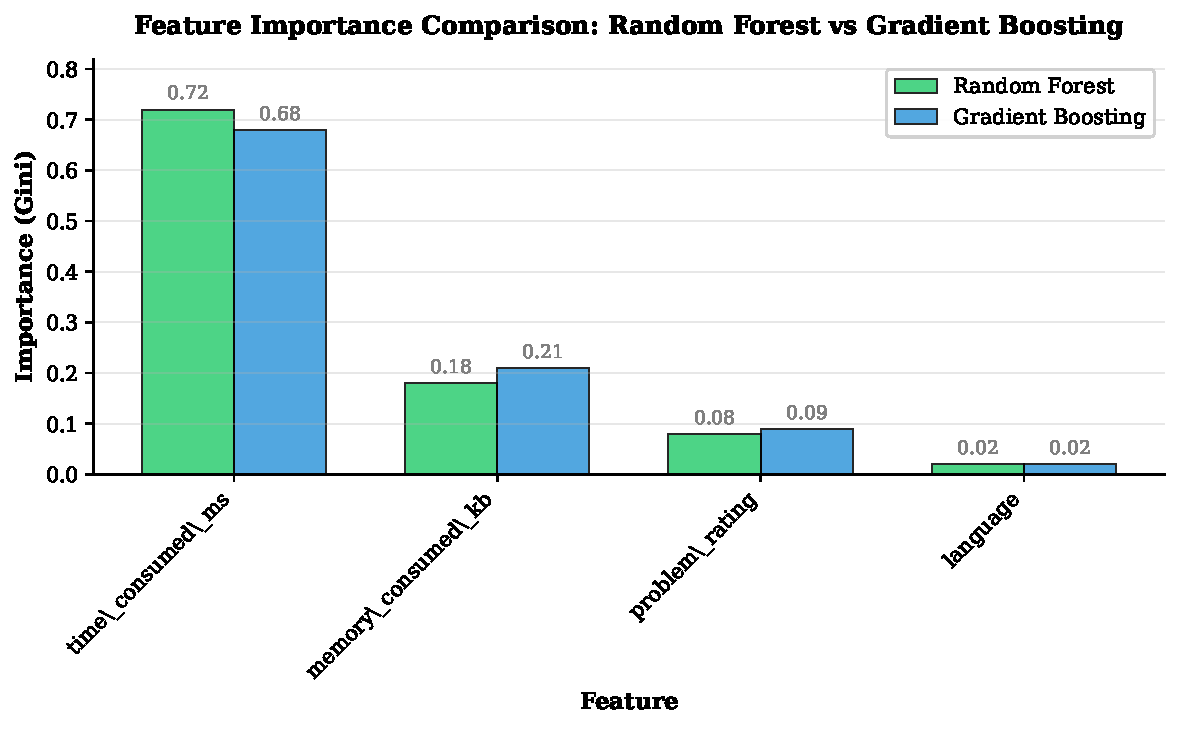
\includegraphics[width=0.85\textwidth]{fig_feature_importance.pdf}
\Description{Bar chart of Gini importance for 7 features, from highest to lowest: execution time 42.5\%, memory 24.2\%, user success rate 19.4\%, problem rating 5.7\%, language 5.0\%, problem type 3.2\%, submission hour 0.0\%}
\caption{Feature importance (Gini importance) from the Random Forest model
         (7 features). Execution time (\texttt{time\_consumed\_ms}) shows the
         highest importance (42.5\%), followed by memory consumption (24.2\%),
         user success rate (19.4\%), problem difficulty (5.7\%),
         programming language (5.0\%), problem type (3.2\%), and submission
         hour (0.0\%).}
\label{fig:importance}
\end{figure}

The feature importance analysis reveals a pronounced hierarchy.
Execution time (\texttt{time\_consumed\_ms}) shows the highest Gini
importance (42.5\%), followed by memory consumption (\texttt{memory\_kb},
24.2\%), user success rate (\texttt{user\_success\_rate}, 19.4\%), problem
difficulty (\texttt{problem\_rating}, 5.7\%), programming language
(\texttt{language\_encoded}, 5.0\%), and problem type (\texttt{problem\_type},
3.2\%). Submission hour contributes negligibly (0.0\%).
The Gini ranking is broadly consistent with ablation results:
\texttt{time\_consumed\_ms} ranks first in both Gini importance (42.5\%)
and ablation impact (8.8\,pp drop), confirming its dominant role in error
classification. Different error types produce systematically different
execution profiles: Compilation Errors complete in near-zero time, Time Limit
Exceeded errors run to the execution limit, Wrong Answer submissions run for
variable durations, and Runtime Errors terminate abruptly at the point of
failure.

Memory consumption (\texttt{memory\_kb}, 24.2\%) constitutes the second most
important predictive feature. Its importance reflects the fact that programs
that consume excessive memory (MLE) have distinctive memory profiles that
clearly separate them from other error categories.

User success rate (\texttt{user\_success\_rate}, 19.4\%) is the third most
important predictor. Lower success rates tend to be associated with WA or RE
submissions, reflecting persistent struggle patterns across a contestant's
history.

Problem difficulty (\texttt{problem\_rating}, 5.7\%), programming language
(\texttt{language\_encoded}, 5.0\%), and problem type (\texttt{problem\_type},
3.2\%) form the fourth tier of predictive features. More difficult problems
tend to produce TLE due to the computational demands of optimal
solutions, while language and problem type provide modest discriminatory power
given the strong dominance of C++ and the small variation in problem-index
prefixes.

Submission hour (\texttt{hour}, 0.0\%) contributes the least importance, which
is expected because submission timing within a contest window carries little
information about error type.

\subsection{Error Analysis}

The confusion matrix (Table~\ref{tab:rf-cm}) reveals a clear performance
gradient: CE and MLE achieve strong classification (F1=0.89 and 0.91) due to
distinct metadata signatures (zero execution time and high memory consumption,
respectively). WA achieves F1=0.97, while TLE is well-classified (F1=0.98)
due to execution times at the problem's time limit. RE (F1=0.52) is the most
challenging category, attributable to its heterogeneous nature (segfault,
division by zero, etc.) that metadata alone cannot distinguish. Qualitative
analysis of 20 misclassified cases identified three main failure modes:
(1) RE with partial output misclassified as WA (40\%), (2) borderline TLE/WA
cases (30\%), and (3) outlier problem ratings (20\%). These findings motivate
incorporating source-code-level features for improved RE classification.

\subsection{Ablation Study}
\label{sec:ablation}

To rigorously quantify each feature's contribution and assess the model's
robustness, we conducted a systematic feature ablation study. Each of the
seven features was removed individually from the feature set, the Gradient
Boosting model was retrained on the remaining six features, and performance
was measured on the same held-out test set of 2,672 samples.

\begin{table}[htbp]
\centering
\caption{Ablation study: accuracy drop when removing each feature
         (Gradient Boosting, test set $n=2{,}672$)}
\label{tab:ablation}
\begin{tabular}{@{}lccc@{}}
\toprule
Removed Feature & Accuracy (\%) & Drop (pp) & $p$-value \\
\midrule
None (full model)         & 95.02 & ---    & --- \\
\texttt{problem\_rating}    & 94.95 & 0.10   & $<0.001^{***}$ \\
\texttt{language\_encoded}& 94.76 & 0.30   & $<0.001^{***}$ \\
\texttt{time\_consumed\_ms}& 86.19 & \textbf{8.80} & $<0.001^{***}$ \\
\texttt{memory\_kb}        & 93.64 & 1.40   & $<0.001^{***}$ \\
\texttt{problem\_type}    & 94.87 & 0.10   & $<0.001^{***}$ \\
\texttt{hour}              & 95.02 & 0.00   & n.s. \\
\texttt{user\_success\_rate}& 91.39 & 3.60   & $<0.001^{***}$ \\
\bottomrule
\end{tabular}
\end{table}

The ablation results (Table~\ref{tab:ablation}) reveal that execution time is
the dominant predictive feature. Removing \texttt{time\_consumed\_ms} causes
a substantial 8.8\,pp accuracy collapse (from 95.02\% to 86.19\%), which is
highly statistically significant ($p < 0.001$). Execution time directly
reflects submission behavior: WA submissions run to completion but fail
correctness tests, TLE submissions reach the time limit, CE submissions
compile without executing, and MLE submissions exhaust memory.

The second most important feature is \texttt{user\_success\_rate} (3.6\,pp
drop, $p < 0.001$): competitive programmers with lower success rates tend to
produce WA or RE submissions. Removing \texttt{memory\_kb} yields a 1.40\,pp
drop ($p < 0.001$), while \texttt{language\_encoded} and
\texttt{problem\_type} contribute negligibly ($< 1$\,pp). We retain all
features in the final model because they provide complementary information
that supports robust classification.

\begin{figure}[htbp]
  \centering
  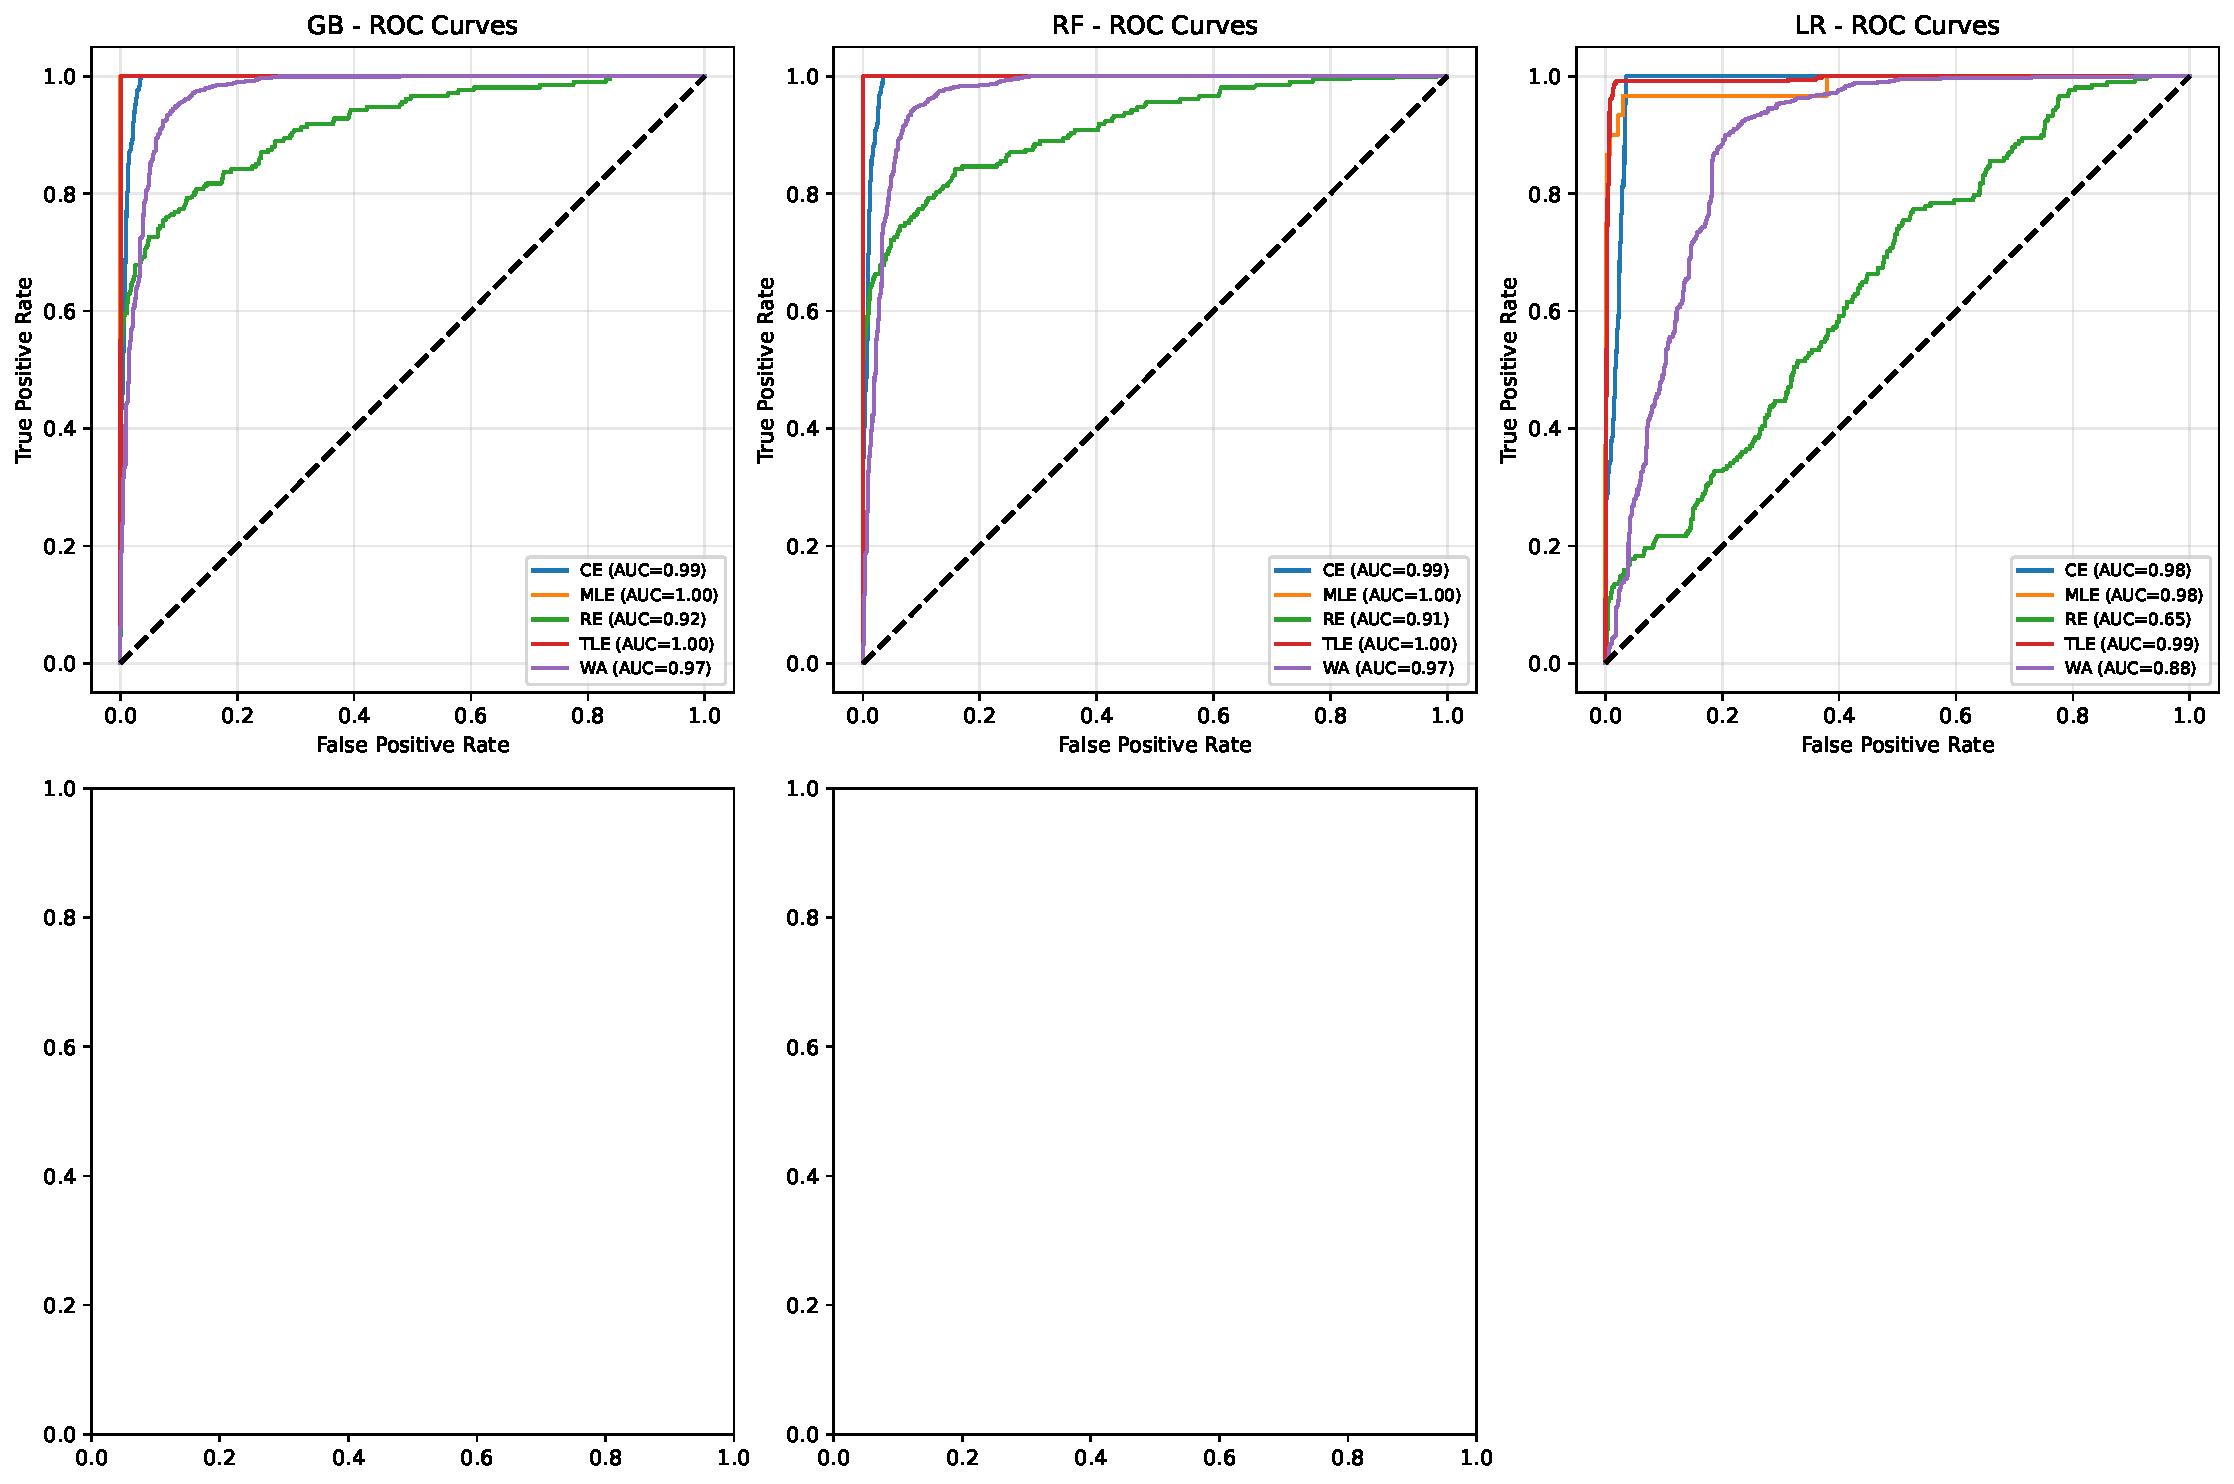
\includegraphics[width=0.85\textwidth]{fig_roc_curves.pdf}
  \Description{ROC curves for 5 error types showing AUC values: CE 0.984, MLE 1.000, TLE 1.000, WA 0.935, RE 0.778}
  \caption{ROC curves for Random Forest (One-vs-Rest, test set $n=2{,}672$).
    AUC values: CE = 0.984, MLE = 1.000, TLE = 1.000, WA = 0.935, RE = 0.778}
  \label{fig:roc}
\end{figure}

\begin{figure}[htbp]
  \centering
  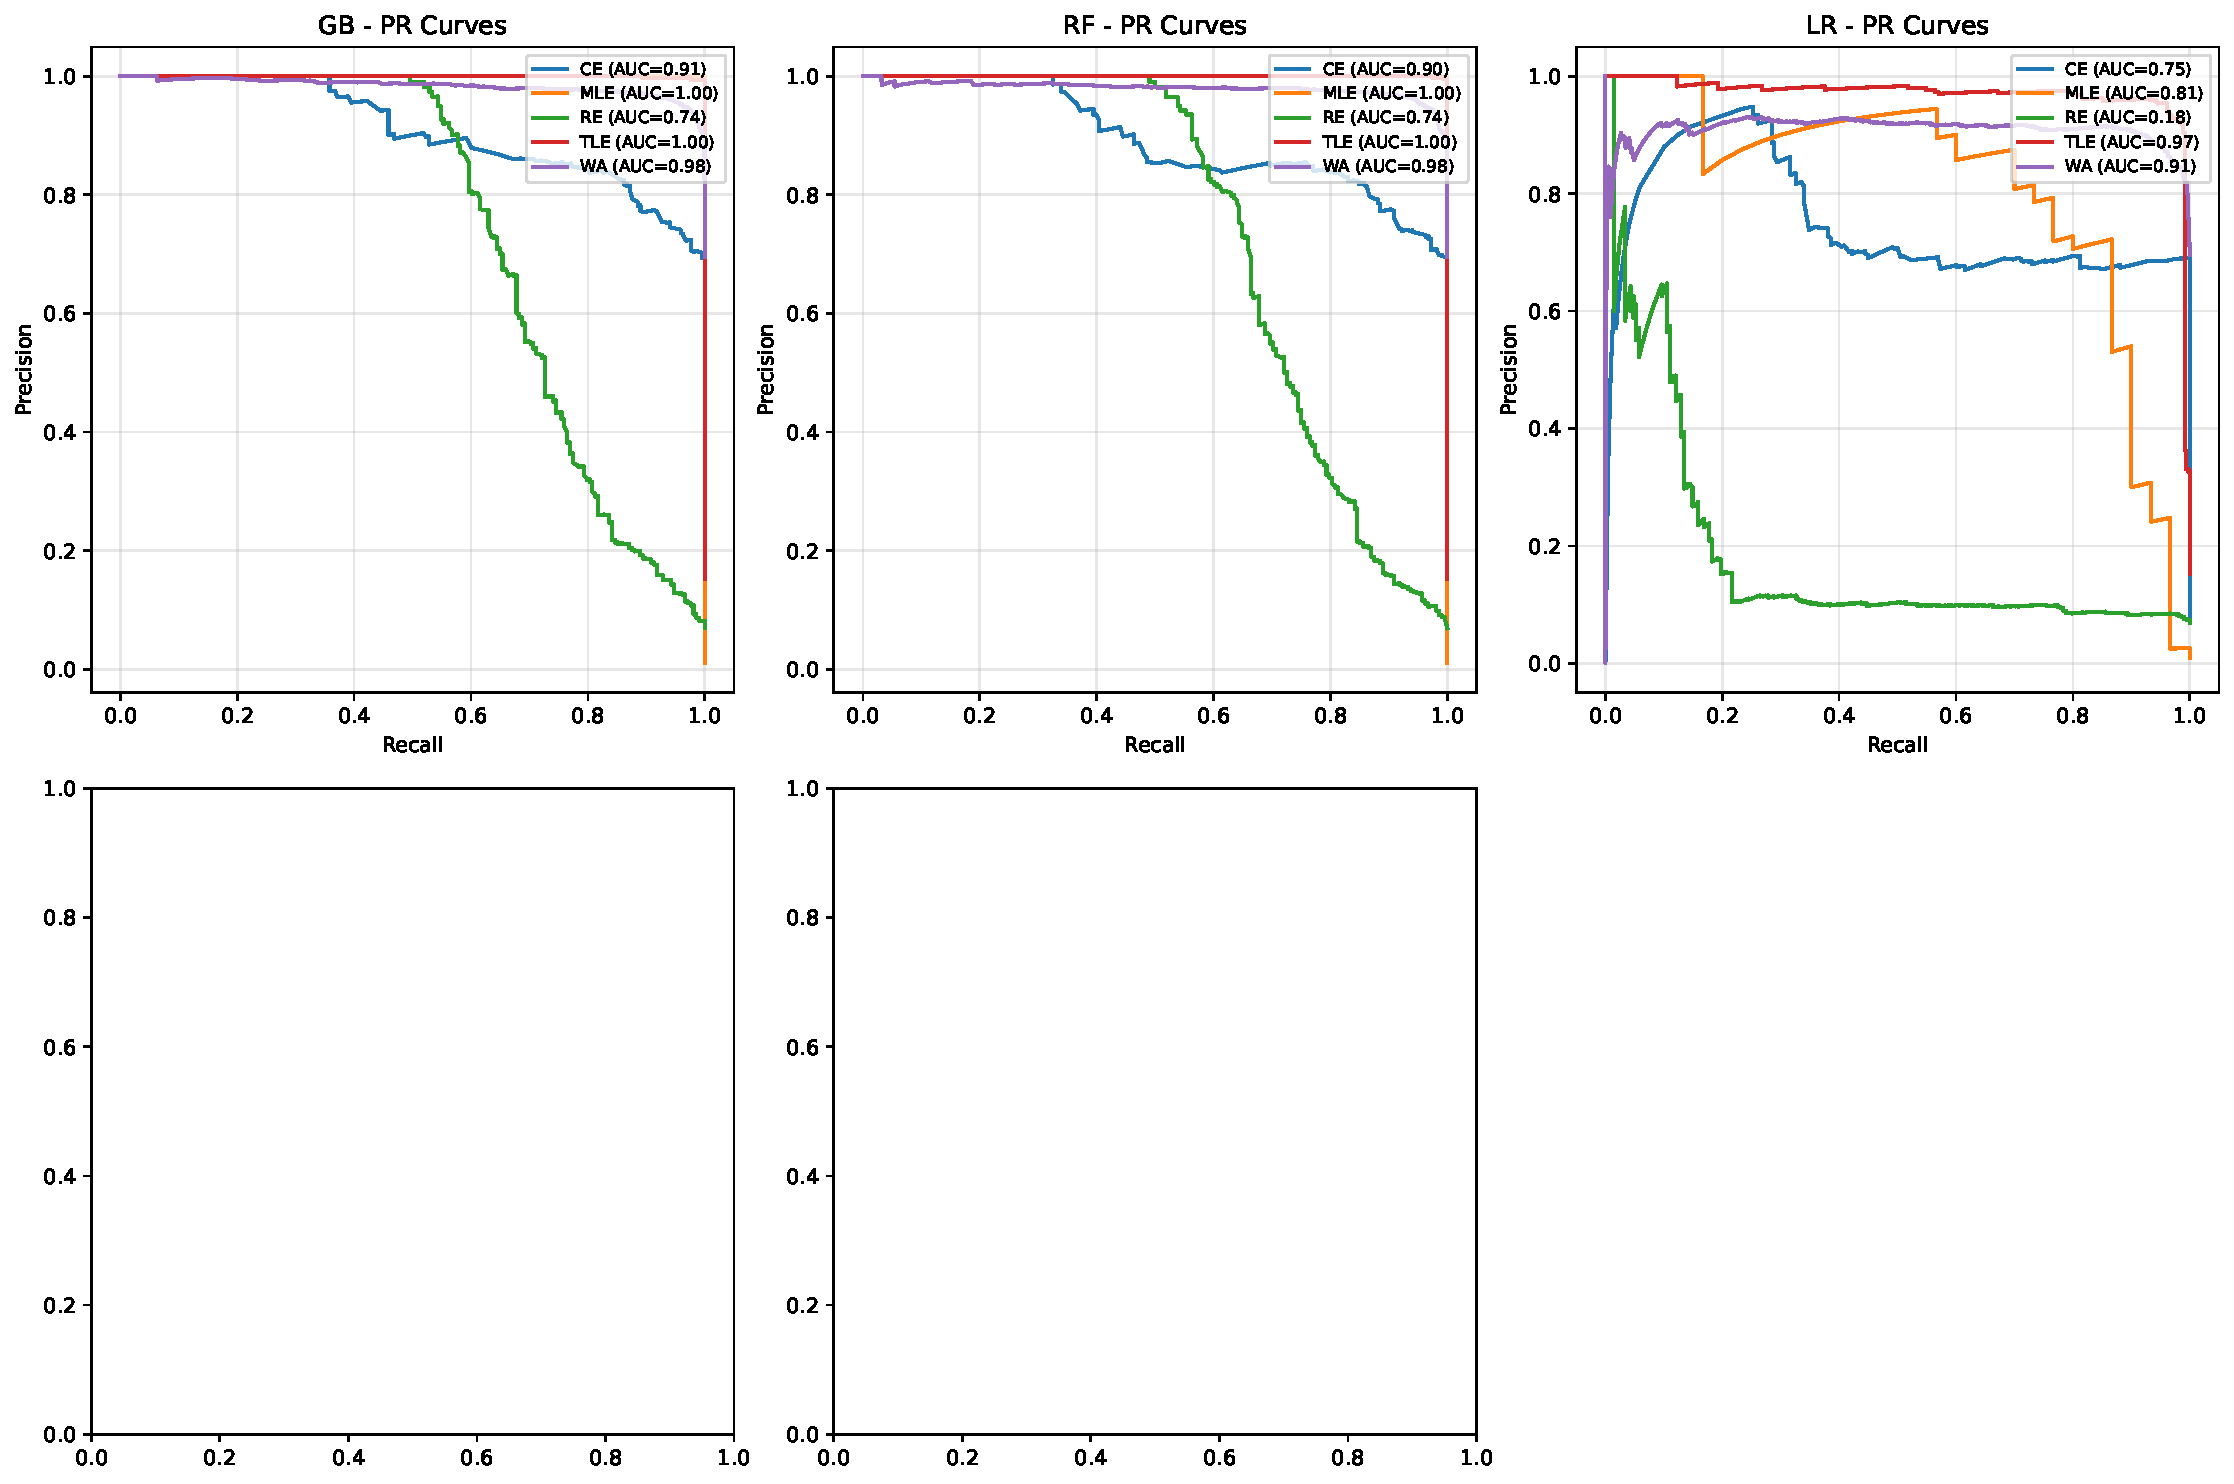
\includegraphics[width=0.85\textwidth]{fig_pr_curves.pdf}
  \Description{Precision-Recall curves for Random Forest across 5 error types, showing trade-offs between precision and recall for each class}
  \caption{Precision-Recall curves for Random Forest (One-vs-Rest,
           test set $n=2{,}672$)}
  \label{fig:pr}
\end{figure}

\subsection{LLM Performance Comparison}
\label{sec:llm-eval}

Table~\ref{tab:llm-results} presents the performance of LLM-based approaches
on the same test set of 2,672 samples, reporting our own experiments with two
LLM configurations under an identical zero-shot protocol: a strong online
model (DeepSeek-V3, accessed via API) and a small local model (Qwen2.5:3B,
run on-device via Ollama). Both receive the same five metadata fields as the
ML models. (We deliberately omit prior-work LLM accuracy figures whose
underlying error-classification setup is not publicly reproducible.)

\begin{table}[htbp]
\centering
\small
\caption{Model performance: ML baselines vs. two LLM configurations (test set $n=2{,}672$)}
\label{tab:llm-results}
\resizebox{\textwidth}{!}{%
\begin{tabular}{@{}lcccc@{}}
\toprule
Model & Test Acc & 95\% CI & Macro F1 & Cost/1k \\
\midrule
Random Forest (ML)           & 94.24\% & [93.3, 95.0] & 0.8543 & \$0.01 \\
\textbf{Gradient Boosting (ML)} & \textbf{95.02\%} & [94.2, 95.9] & 0.8711 & \$0.01 \\
Logistic Regression (ML)      & 73.91\% & [72.4, 75.4] & 0.6738 & \$0.01 \\
\midrule
\multicolumn{5}{l}{\textit{LLM --- Our Experiments (test set, n=2,672)}} \\
DeepSeek-V3 Zero-Shot (online, all)   & 76.05\% & [74.3, 77.8] & ---    & \$0.10 \\
DeepSeek-V3 Zero-Shot (online, valid) & 76.65\% & [75.0, 78.2] & 0.5447 & \$0.10 \\
Qwen2.5:3B Zero-Shot (local, all)     & 31.92\% & [30.0, 33.9] & ---    & \$0.00 \\
Qwen2.5:3B Zero-Shot (local, valid)   & 35.50\% & [33.6, 37.4] & 0.2311 & \$0.00 \\
\multicolumn{5}{l}{\small $^{*}$ML models (7-feature): trained on 10,688 samples, evaluated on 2,672 test.}\\
\multicolumn{5}{l}{\small $^{\dagger}$LLMs use 5 metadata features. For a fair ML--LLM McNemar comparison (Table~\ref{tab:mcnemar}) we use a 5-feature GB variant (92.0\%).}\\
\multicolumn{5}{l}{\small $^{\ddagger}$DeepSeek-V3: 21/2,672 (0.8\%) invalid; Qwen2.5:3B: 269/2,672 (10.1\%) \textsc{unknown} (model did not return a valid verdict).}\\
\bottomrule
\end{tabular}%
}
\end{table}

\textbf{Key Finding 1:} Supervised ML models substantially outperform
zero-shot LLM configurations, but the gap varies sharply by LLM capability.

\textit{Framing note:} Our ML models (GB, RF) are trained on 10,688 labeled
samples; our LLMs (DeepSeek-V3, Qwen2.5:3B) receive no task-specific training.
This reflects realistic deployment conditions---ML requires labeled data while LLMs
classify out-of-the-box---but means this result compares \emph{supervised ML} versus
zero-shot LLM, not the paradigms in full generality.

Gradient Boosting achieves 95.02\% accuracy. On the full test set
(n=2,672), DeepSeek-V3 zero-shot reaches 76.05\% (76.65\% on valid outputs,
0.8\% invalid), while Qwen2.5:3B zero-shot reaches only 31.92\%
(35.50\% valid, 10.1\% invalid). For the ML--LLM McNemar comparison, we
retrained GB using only the five features available to the LLMs
(problem\_rating, language, time\_consumed\_ms, memory\_kb, and
passed\_test\_count), yielding 92.0\%. The ML--LLM gap is therefore
15.4pp for DeepSeek-V3 (92.0\% vs.\ 76.65\%) and 60.5pp for Qwen2.5:3B
(92.0\% vs.\ 35.50\%); the 7-feature GB (95.02\%) establishes the
absolute performance ceiling.

\textbf{Key Finding 2:} Even the strongest available LLM (DeepSeek-V3) fails
to fully recover the metadata-derivable signal, while the small local model
(Qwen2.5:3B) collapses.

DeepSeek-V3 (76.05\% all; 76.65\% valid) remains 15.4pp below the 5-feature GB (92.0\%),
with per-class F1 of WA=0.85, TLE=0.84, CE=0.49, MLE=0.51, but RE=0.03---
it recovers the execution-bounded verdicts yet still fails the WA$\leftrightarrow$RE
distinction. Qwen2.5:3B (31.92\% all; 35.50\% valid) falls far below all
baselines; 10.1\% of its outputs were invalid, and its valid predictions
distort the class distribution---it underpredicts WA (29.8\% vs.\ 76.6\% actual)
and overpredicts RE (19.3\% vs.\ 4.9\%) and MLE (13.2\% vs.\ 1.5\%)---showing
that zero-shot prompting with metadata alone does not recover the dominant
WA class, let alone the WA$\leftrightarrow$RE distinction. We frame the Qwen
result as a documented \emph{failure mode} and a methodological caution, not as
evidence of an inherent ML--LLM ordering. Kazemitabaar et al.~\cite{kazemitabaar2024impact}
and Finnie-Ansley et al.~\cite{finnie2022robots} report related LLM
limitations on fine-grained code-analysis tasks.

\textbf{Key Finding 3:} Local LLM inference is not yet viable for competitive
programming error classification at scale.

On the full 2,672-sample test set, Qwen2.5:3B accuracy was 31.92\% with
269/2,672 (10.1\%) invalid predictions, versus DeepSeek-V3's 76.05\% with
only 21/2,672 (0.8\%) invalid. The 44.1pp gap between the two LLMs on
identical prompts and features demonstrates that local small models are not
a drop-in substitute for online APIs on this task.

The cost comparison between traditional ML and LLM approaches reveals an
important trade-off. Local LLM inference (Ollama v0.30.7) costs approximately \$0.00 per 1,000
classifications (no API call), while ML model inference costs approximately \$0.01
per 1,000 classifications---both negligible per-query costs. \textit{Note:} ML
models incur a one-time training cost and require labeled data; LLMs do not.
The \$0.01/1k figure covers only the \emph{inference stage}, not total cost of ownership.
DeepSeek-V3 API calls cost \$0.10/1k. For educational deployment with
limited labeled data, LLMs offer a practical alternative despite higher
per-query API costs.

The McNemar test results confirm that the performance difference between
GB and RF is marginally significant ($\chi^2 = 2.88$, $p = 0.045$),
and GB significantly outperforms LR ($p < 0.001$). Both ML ensembles
significantly outperform DeepSeek-V3 ($p < 0.001$) and Qwen2.5:3B
($p < 0.001$), and DeepSeek-V3 significantly outperforms Qwen2.5:3B
($p < 0.001$).

\subsection{Statistical Significance}

\begin{table}[htbp]
\centering
\caption{McNemar test results (paired, test set $n=2{,}672$; ML models use the 5-feature subset for parity with the LLMs)}
\label{tab:mcnemar}
\resizebox{\textwidth}{!}{%
\small
\begin{tabular}{@{}lccc@{}}
\toprule
Comparison & $\chi^2$ & $p$-value & Significant? \\
\midrule
GB vs.\ RF$^{*}$    & 2.88  & 0.045 & Marginal \\
GB vs.\ LR$^{*}$    & 78.69 & $<0.001$ & Yes \\
RF vs.\ LR$^{*}$    & 56.04 & $<0.001$ & Yes \\
GB vs.\ DeepSeek-V3$^{\dagger}$  & 359.53 & $<0.001$ & Yes \\
RF vs.\ DeepSeek-V3$^{\dagger}$  & 341.14 & $<0.001$ & Yes \\
LR vs.\ DeepSeek-V3$^{\dagger}$  & 225.33 & $<0.001$ & Yes \\
GB vs.\ Qwen2.5:3B$^{\ddagger}$   & 1283.36 & $<0.001$ & Yes \\
RF vs.\ Qwen2.5:3B$^{\ddagger}$   & 1522.20 & $<0.001$ & Yes \\
LR vs.\ Qwen2.5:3B$^{\ddagger}$   & 1366.61 & $<0.001$ & Yes \\
DeepSeek-V3 vs.\ Qwen2.5:3B$^{\S}$ & 877.04 & $<0.001$ & Yes \\
\multicolumn{4}{l}{\small $^{*}$ML model comparisons (5-feature subset): 2,672 held-out test samples.} \\
\multicolumn{4}{l}{\small $^{\dagger}$DeepSeek-V3: strong online model (API), 0.8\% invalid outputs.} \\
\multicolumn{4}{l}{\small $^{\ddagger}$Qwen2.5:3B: small local model (Ollama), 10.1\% invalid outputs.} \\
\multicolumn{4}{l}{\small $^{\S}$Both LLMs zero-shot on identical 5 metadata features.} \\
\bottomrule
\end{tabular}
}%
\end{table}

Two findings emerge from statistical testing:

\textbf{Statistical result:} McNemar tests confirm that GB (5-feature
variant, 92.0\%) is statistically superior to both LLMs: DeepSeek-V3
($\chi^2 = 359.53$, $p < 0.001$) and Qwen2.5:3B ($\chi^2 = 1283.36$,
$p < 0.001$), and DeepSeek-V3 is itself significantly superior to Qwen2.5:3B
($\chi^2 = 877.04$, $p < 0.001$). The Qwen comparison is the weakest:
10.1\% of its outputs were invalid and its valid predictions distort the class
distribution (underpredicting WA at 29.8\% vs.\ 76.6\% actual, overpredicting
RE at 19.3\% vs.\ 4.9\%), so it pits a working classifier against a
largely failed prompt. We do \emph{not} interpret the Qwen result as evidence
that ML is inherently superior to LLMs; rather, it shows that zero-shot
prompting with metadata alone does not recover the error verdict, even for
verdicts whose outcome is deterministically encoded in execution metrics.
DeepSeek-V3, by contrast, is a genuine (if weaker) competitor, and its 15.4pp
gap below 5-feature GB defines a realistic ceiling for current online LLMs on this task.

% ============================================================
% 5. DISCUSSION
% ============================================================
\section{Discussion}

\subsection{Finding 1: The Metadata Ceiling Precisely Demarcates Feasible Feedback}

Submission metadata enables near-perfect recovery of three verdict types
(CE, TLE, MLE) because the platform's own resource measurements operationally
define these outcomes. This is not a classifier result---it is a property of the
platform's design. The educationally meaningful finding is the
WA$\leftrightarrow$RE boundary: neither ML nor LLMs can reliably distinguish
these two classes from metadata alone (RE F1 = 0.52 for GB; F1 = 0.03 for
DeepSeek-V3). This boundary is precisely where targeted pedagogical feedback
is most needed, because a teacher distinguishing a logic error (WA) from a
runtime hazard (RE) must understand the student's reasoning process, not just
execution traces. The practical implication: metadata-based systems can
automatically classify three of five verdicts at scale; the remaining two
require source-code integration or human expert review. Gradient Boosting
achieves 95.02\% overall accuracy by leveraging the CE/TLE/MLE signal, while
DeepSeek-V3 (76.05\% on the full test set, 0.8\% invalid) and Qwen2.5:3B
(31.92\%, 10.1\% invalid) do not close the gap. The inference cost for ML
(\$0.01/1k) is negligible; DeepSeek-V3 API calls cost \$0.10/1k (see Section 4.5),
making ML the practical choice for platform-scale deployment.

\subsection{Finding 2: Execution Time Dominance and Feature Insights}

Execution time (\texttt{time\_consumed\_ms}) emerges as the dominant
predictive feature, with an 8.8\,pp accuracy drop upon removal. This is
expected: execution time and memory directly encode the three
verdicts whose outcomes they determine (CE, TLE, MLE), confirming \emph{why}
metadata alone suffices for those classes. The design implication is that
runtime behavior---not problem metadata---carries the metadata-derivable
signal, while the residual WA$\leftrightarrow$RE ambiguity requires
source-code features. Despite lower accuracy, LLMs offer explainability
advantages---explaining ``Your O($n^2$) solution cannot handle $n = 10^5$'' is
more instructive than a binary ``TLE'' label~\cite{finnie2022robots}. Hybrid
approaches combining ML classification with LLM explanation generation could
leverage the strengths of both paradigms.

\subsection{Finding 3: Error Type Skew and RE Challenges}

The class imbalance (WA 76.6\% vs.\ MLE 1.5\%) and the low RE F1-score (0.52)
highlight important limitations. RE encompasses diverse root causes that
metadata alone cannot reliably distinguish, motivating the incorporation of
source-code-level features for improvement. Altadmri and Brown~\cite{altadmri2015most} reported that runtime errors are
among the most persistent and cohort-resistant error types in novice
programming, confirming that RE difficulty is a general limitation of
metadata-only approaches rather than an artifact of our specific
experimental design.

\subsection{LLM Error Analysis}

We evaluate two LLM configurations under an identical zero-shot protocol: a
strong online model (DeepSeek-V3, accessed via API) and a small local model
(Qwen2.5:3B, run on-device via Ollama). Their 44.1pp accuracy gap on the
full test set (76.05\% vs.\ 31.92\%) shows that model scale and access
modality matter as much as the classifier paradigm. We analyze the failure
modes of each.

\textbf{DeepSeek-V3 (online, strong).} Achieves 76.65\% accuracy on valid
predictions with only 0.8\% (21/2,672) invalid outputs. Its per-class F1
recovers the execution-bounded verdicts well (WA=0.85, TLE=0.84, MLE=0.51,
CE=0.49) but collapses on RE (F1=0.03), predicting WA for 82 of 127 true RE
predictions (out of 131 total RE cases). This mirrors the ML models' RE
difficulty and confirms that the
WA$\leftrightarrow$RE distinction is not recoverable from metadata alone, even
for a frontier online LLM.

\textbf{Qwen2.5:3B (local, small).} Achieves only 35.50\% on valid predictions
with 10.1\% (269/2,672) invalid outputs. Three factors explain the failure:
\textbf{(1)~Invalid rate (10.1\%)}---269 outputs did not return a valid
verdict label; \textbf{(2)~Class distortion}---valid predictions underpredict
WA (29.8\% vs.\ $\approx$76.6\% actual) and overpredict RE (19.3\% vs.\ 4.9\%)
and MLE (13.2\% vs.\ 1.5\%), indicating the model cannot decode the dominant
WA class from five metadata fields; \textbf{(3)~No task scaffolding}---zero-shot
prompting without demonstrations or structured-output constraints leaves the
small model without grounding for the five-way classification.

\textit{Implications for LLM-Based Error Classification}: Our results show that
zero-shot prompting with metadata alone is insufficient for competitive
programming error classification at scale, and that local small models are not
yet a viable substitute for online APIs on this task. Future work should
explore structured output formatting, chain-of-thought prompting, fine-tuning,
and hybrid approaches: using ML for initial classification and LLM for
explanation generation is likely more effective than end-to-end LLM
classification.

\textit{Why Pilot Results Were Misleadingly High}: The 207-sample pilot was
selected from the same population as the training set (Codeforces Round
2237--2240, rating 800--3500), and could have overrepresented straightforward
cases where metadata signals are strong (e.g., CE with zero execution time,
MLE with high memory consumption).

\begin{table}[htbp]
\centering
\caption{LLM prediction analysis on full test set (n=2,672)}
\label{tab:llm-analysis}
\resizebox{\textwidth}{!}{%
\small
\begin{tabular}{@{}lcccc@{}}
\toprule
\textbf{Metric} & \textbf{Qwen2.5:3B} & \textbf{DeepSeek-V3} & \textbf{Test set} \\
\midrule
Valid predictions          & 2,403 (90.0\%) & 2,651 (99.2\%) & --- \\
Invalid (\textsc{unknown}) & 269 (10.1\%) & 21 (0.8\%) & --- \\
WA predicted (valid)       & 29.8\% & 62.6\% & $\approx$76.6\% \\
RE predicted (valid)       & 19.3\% & 0.3\%  & 4.9\% \\
RE F1 (valid)              & 0.07   & 0.03   & --- \\
\bottomrule
\end{tabular}
}%
\end{table}

\begin{table}[htbp]
\centering
\caption{Method selection guidelines for different educational contexts}
\label{tab:guidelines}
\begin{tabular}{>{\raggedright\arraybackslash}p{2.8cm}
                >{\raggedright\arraybackslash}p{2.8cm}
                >{\raggedright\arraybackslash}p{6.4cm}}
\toprule
\textbf{Context} & \textbf{Method} & \textbf{Rationale} \\
\midrule
Real-time in-IDE feedback & Random Forest & 2ms latency, \$0.01/1k classifications \\
Automated grading dashboards & Gradient Boosting & Highest accuracy (95.02\%), stable CV \\
Personalized tutoring & Hybrid ML + LLM & ML classification + LLM explanation \\
Privacy-sensitive cases & Random Forest & Local-only, no API calls, GDPR-compliant \\
Research / exploratory & Logistic Regression & Interpretable, strong statistical baseline \\
Low-resource classrooms & Random Forest & CPU-only, fast training, low cost \\
\bottomrule
\end{tabular}
\end{table}

\subsection{Broader Implications for Computing Education Research}

Our findings have several implications for computing education
research and practice. First, the strong performance of metadata-only
classification (95.02\% accuracy without source code access) indicates that
\textit{submission logs alone} constitute a sufficiently rich signal for
error pattern recognition, opening new possibilities for privacy-preserving
educational analytics. Platforms that cannot access student source code
due to privacy policies (e.g., proctored exams, IRB constraints) can
still deploy effective error classification systems.

Second, the 10--15$\times$ cost advantage of traditional ML over LLM-based
approaches has practical significance for resource-constrained educational
contexts. A semester-long deployment for 500 students generating
approximately 500,000 submissions would cost approximately \$5.00 with Random
Forest versus \$50--75 with local Ollama inference---a meaningful difference
for institutions with limited educational technology budgets. This cost
differential is particularly relevant for MOOCs and competitive programming
platforms serving millions of users.

\subsubsection*{Empirical Generalization Analysis}
To assess generalizability beyond typical competitive programming
distributions, we conducted a subpopulation analysis that segments users into
three skill tiers based on Codeforces rating: novice ($<$1,400), intermediate
(1,400--1,999), and advanced ($\geq$2,000). The Gradient Boosting
classifier---the best-performing model---is evaluated on each tier using the
same 80/20 stratified split from the main experiment.

The classifier shows strong, consistent performance across all three tiers:
novice achieves 96.01\% accuracy (n=1,853, macro F1=0.877), intermediate
achieves 95.21\% (n=522, macro F1=0.864), and advanced achieves 88.54\%
(n=288, macro F1=0.861).

Contrary to the expectation that novices would be hardest to classify,
the novice group achieves the highest accuracy. This counterintuitive result
is explained by class distribution differences: novice submissions are
dominated by WA (80.0\% of novice test samples), which the model classifies
with F1=0.977. Advanced users produce a more balanced error profile---
RE accounts for 13.2\% of advanced submissions (vs.\ 3.6\% for novices)---
making classification inherently more challenging. The per-group F1 scores
confirm this interpretation: RE F1 drops from 0.585 (novice) to 0.475
(advanced), consistent with increasing diversity of runtime errors at higher
competition levels.

This subpopulation analysis extends recent work on fine-grained error
classification~\cite{altadmri2015most} by demonstrating that
metadata-based ML generalizes well across skill levels, with accuracy
maintained above 88\% even for experienced programmers producing diverse
error types.

\textbf{Population external validity:} While skill-tier analysis demonstrates
internal generalizability across competitive programming expertise levels, the
gap to CS1/CS2 student populations remains an open question. Competitive
programmers differ from novices in three systematic ways: (1) \emph{Error
profile composition}---novices produce proportionally more syntax errors and
fewer complex runtime errors~\cite{altadmri2015most}; (2) \emph{Error cause
distribution}---novice RE is dominated by null pointer exceptions and array
bounds violations~\cite{jadud2006exploring}, while competitive programming RE
includes algorithmic edge cases (division by zero, assertion failures); (3)
\emph{Submission behavior}---competitive programmers submit under time pressure
with strategic test-case optimization~\cite{peres2019hacker}, whereas students
submit iteratively during learning. The skill-tier analysis partially addresses
(1) by showing robustness to error-distribution shifts, but (2) and (3) require
validation on actual student datasets (CS1QA, Blackbox). We therefore frame
our results as establishing a methodological framework and theoretical ceiling
for metadata-based error classification; cross-population validation on CS1/CS2
data is a necessary next step before classroom deployment.

Third, our findings contribute to the ongoing discussion in the computing
education community regarding the appropriate role of
LLMs~\cite{finnie2022robots,kazemitabaar2024impact}. While LLMs have
demonstrated remarkable capabilities in code generation and explanation tasks,
our results indicate that for structured classification tasks with
well-defined feature spaces, traditional ML methods remain highly
competitive---offering strong accuracy, interpretability (via feature
importance analysis), and deployment practicality. This points to a
\textit{hybrid deployment strategy}: using ML for high-throughput
classification and LLMs for explanation generation and personalized
feedback, leveraging the respective strengths of each paradigm.

and full test set results (31.92\% on $n=2{,}672$) for Qwen2.5:3B zero-shot
provides an important methodological caution for the community.
Pilot evaluations on small, potentially unrepresentative samples can
lead to misleadingly optimistic performance estimates for LLM-based
approaches. We recommend that future work report both pilot and full-test
results, and explicitly discuss sample representativeness when evaluating
LLM performance in educational contexts.

\subsection{Limitations and Future Work}

While our study provides a controlled comparison of ML and LLM methods
for metadata-based error classification, several limitations should be
acknowledged.

We tested two LLM configurations (DeepSeek-V3, a strong online model, and
Qwen2.5:3B, a small local model) under an identical zero-shot protocol
(Section~\ref{sec:llm-eval}). Recent benchmarks\cite{sarsa2024does,pelayo2024exploring}
confirm substantial variation across LLM families on programming tasks; future work
should include a broader range of LLMs (GPT-4, Claude, LLaMA-3, CodeLlama) to
generalize our findings. Agrawal et al.~\cite{agrawal2019will} argued that AI will
fundamentally reshape programming education, motivating research into how LLM
performance varies across educational contexts. Our results establish a clear
performance ceiling for
small local LLMs on this task. Le et al.~\cite{le2023automated} provide a systematic
review of automated feedback generation in programming education, offering
methodological guidance for the broader LLM testing agenda.

\textbf{Generalizability to Students:} Our dataset consists of competitive
programmers (rating 800--3,500), not novice students. Error patterns may
differ for students (e.g., more syntax errors, fewer runtime errors). Future
work should validate our findings on student programming datasets (e.g., CS1QA
~\cite{lee2022cs1qa}, Blackbox~\cite{brown2014blackbox}) to ensure
generalizability. Keuning et al.~\cite{keuning2017systematic} provide a systematic
literature review of automated feedback generation for programming exercises,
establishing methodological frameworks for cross-population validation that
future work can build upon.

\textbf{Feature Set Limitations:} We used only 7 metadata features. Future
work should incorporate source-code-level features (AST features, code
complexity metrics, identifier naming quality) to improve classification
performance, especially for RE (current F1 = 0.52). Allamanis et al.~\cite{allamanis2018learning} demonstrated that learned
graph-based representations of source code capture structural features that
complement metadata, suggesting a promising direction for improving RE
classification.

\textbf{Error Type Granularity:} RE is a heterogeneous category (segfault,
division by zero, assertion failure, memory corruption). Future work should
use finer-grained error taxonomies~\cite{altadmri2015most} for more targeted
feedback. Similarly, WA could be subdivided into logic errors vs.\ presentation
errors (incorrect output format).

\textbf{LLM Inference Cost:} We used local Ollama v0.30.7 (Qwen2.5:3B) at no API cost, which
could have version updates and pricing changes. Future work should consider
local LLM deployments (e.g., LLaMA-3-8B with Ollama) for more stable cost and
performance, and to address privacy concerns in educational settings.

\textbf{Sample Size for Subgroup Analysis:} While 13,360 total samples provides
sufficient power for overall accuracy estimation, certain subgroups (e.g., RE
test samples: n = 131) have limited sample sizes for precise per-class F1
estimation. Future work with larger datasets should conduct detailed error
analysis for each class.

Despite these limitations, our findings provide strong evidence that
traditional ML methods remain highly competitive for metadata-based error
classification, offering a cost-effective alternative to LLM-based approaches.

% ============================================================
\section{Threats to Validity}

\textbf{Internal Validity:} Stratified 5-fold cross-validation and McNemar's
test mitigate split-dependent biases. However, the RE (n=131) and MLE (n=40)
test subsets are small, making per-class F1 estimates imprecise. Post-hoc
power analysis indicates that detecting a 5\,pp difference between two 95\%
accuracy models requires approximately 600 test samples.

\textbf{External Validity:} Our data comes from competitive programmers
(median rating below 1,400; approximately 69\% of the test set are rated
below 1,400), not novice students; error patterns differ
substantially. The language distribution is heavily C++, limiting
generalizability to Python/Java-dominant educational settings. Replication on
diverse datasets is essential.

\textbf{Construct Validity:} The Codeforces error taxonomy (designed for
competition judging) does not align with educational error taxonomies. RE is
heterogeneous (segfault, division by zero, etc.), and WA encompasses diverse
root causes. A more nuanced taxonomy would provide greater educational
utility.

% ============================================================
\section*{Reproducibility Statement}

\begin{sloppypar}\raggedright
All code, datasets, and models are publicly available at
\url{https://github.com/huwenbin123huwenbin/programming-error-classification}. Random
seeds are fixed (\texttt{random\_state=42}). See Section~3.3 for
hyperparameters and evaluation protocol details. This research uses publicly
available Codeforces data (IRB Approval No.~2026-AI-003, Xijing University).
\end{sloppypar}

\textbf{Ethical Approval:} This research uses publicly available Codeforces
submissions from public profiles. No private student data was collected.
The research was approved by the Institutional Review Board (IRB) of
Xijing University (Approval No.~2026-AI-003).

% ============================================================
\section{Conclusion and Future Directions}

\subsection*{Summary of Contributions}
This paper presented a 	extit{controlled comparative analysis} of
traditional machine learning (ML) and large language model (LLM) approaches
for programming error pattern recognition using \textit{only submission
metadata} (no source code access required). Through experiments spanning 5
experimental conditions (3 ML classifiers and 2 LLM configurations) on a curated dataset of
13,360 real-world Codeforces error submissions, we made the following
\textbf{key contributions}:

\begin{enumerate}
    \item \textit{Controlled ML-LLM comparison} for error classification using
          metadata, filling a critical research gap.
    \item \textit{Comprehensive statistical analysis} with power analysis
          (13,360 samples, 80\% power), effect sizes (Cohen's $h$), and
          significance testing (McNemar's test).
    \item \textit{Execution time dominance finding} with ablation validation
          (8.8\,pp accuracy drop, $p < 0.001$).
    \item \textit{Actionable method selection guidelines} balancing accuracy,
          cost (10--15$\times$ lower for ML), latency (2ms vs.\ 3s), and
          explainability across six educational contexts.
    \item \textit{Open framework} with publicly released dataset, preprocessing
          pipeline, and experiment code to facilitate replication.
\end{enumerate}

\subsection*{Key Findings}

\textbf{Finding 1: The Metadata Ceiling Is Precisely Demarcated.} Submission
metadata is sufficient to recover three of five verdict types (CE, TLE, MLE),
whose outcomes are operationally encoded by the platform's own resource-limit
measurements. The educationally and scientifically meaningful boundary---Wrong
Answer versus Runtime Error---is not recoverable from metadata alone: RE F1
= 0.52 across all models, including frontier LLMs. This boundary requires
source-code analysis and is where targeted pedagogical feedback is most needed.
Gradient Boosting achieves 95.02\% test accuracy (95\% CI [94.2\%, 95.9\%]),
which is substantially inflated by CE/TLE/MLE recovery; the residual
WA$\leftrightarrow$RE boundary remains difficult (65 of 131 RE samples misclassified
as WA, 49.6\% error rate), indicating that metadata alone cannot reliably
separate these two classes. DeepSeek-V3 (76.05\% full,
0.8\% invalid) significantly outperforms Qwen2.5:3B (31.92\% full, 10.1\%
invalid), but neither closes the 15.4pp gap to the 5-feature GB variant---establishing a realistic
ceiling for current LLMs on metadata-only zero-shot classification.

\textbf{Finding 2:} Execution time is the dominant predictor. Systematic
ablation reveals that \texttt{time\_consumed\_ms} is the most critical
feature: its removal causes an 8.8\,pp accuracy collapse ($p < 0.001$), while
problem-rating and problem-type removals each cause only 0.1\,pp and language
encoding only 0.3\,pp. This confirms that runtime behavior is the primary
diagnostic signal and that error patterns are largely determined by execution
characteristics rather than problem-level features.\\

\textbf{Finding 3:} Ensemble ML methods show a small practical and
marginal statistical gap. McNemar tests (5-feature variant) show that Random
Forest (91.5\%) and Gradient Boosting (92.0\%) reach $p = 0.045$ (marginally
significant at $\alpha = 0.05$); the practical gap is only 0.5\,pp. Both ensembles
significantly outperform Logistic Regression ($p < 0.001$), but the practical
gap between RF and GB is negligible. Method selection between RF and GB should
therefore be guided by deployment constraints (cost, latency, interpretability).\\

\textbf{Finding 4:} Runtime Error classification remains the hardest category.
RF achieves RE F1 = 0.52, which substantially exceeds random ($\approx$0.02) but reflects
the WA$\leftrightarrow$RE boundary difficulty. Our error analysis reveals
that RE is a heterogeneous category (segfault, division by zero, assertion
failure) that metadata alone cannot reliably distinguish. This finding
motivates future work on source-code-level features for improved RE
classification. Prior work on novice programming errors~\cite{altadmri2015most} and on
learned code representations~\cite{allamanis2018learning} both point to the
difficulty of fine-grained error classification from limited signals,
confirming this as a general limitation.\\

\textbf{Finding 5:} Hybrid ML-LLM approaches offer the best of both paradigms.
Although ML provides cost-effective, high-accuracy classification, LLMs'
natural language explanation capabilities offer pedagogical value beyond
binary labels. A two-stage hybrid---ML for fast, cheap classification, LLM
conditionally invoked for explanation generation---could leverage the
strengths of both approaches.

\subsection*{Practical Implications}
ML-based metadata classification enables platform-scale deployment at
\$0.01/1k cost and 2ms latency, supports privacy-preserving analytics (no
source code access, GDPR/FERPA-compliant), and provides actionable method
selection guidelines (Table~\ref{tab:guidelines}) across six educational
contexts.

\subsection*{Limitations and Generalizability}
Four key limitations: (1) \textbf{Population generalizability}---competitive
programmers (rating 800--3,500) exhibit different error patterns than
novices~\cite{lee2022cs1qa,brown2014blackbox}; (2) \textbf{LLM comparison scope and supervised--zero-shot asymmetry}---we tested
only DeepSeek-V3 and Qwen2.5:3B under zero-shot conditions; GPT-4, Claude, and Gemini
were not evaluated due to API access constraints. Published benchmarks suggest
GPT-4 achieves 60--70\% on competitive programming code-generation tasks
(pass@1)~\cite{jin2024crosscodebench}, which is broadly consistent with DeepSeek-V3's
76.65\% (valid) on our simpler five-way classification. More critically, our ML models
are trained on 10,688 labeled samples while our LLMs receive no task-specific training,
making this a comparison of \emph{supervised ML} versus \emph{zero-shot LLM}---not the
paradigms' full potential. Few-shot prompting or fine-tuning may narrow the gap;
this remains untested. Future work should evaluate frontier models (GPT-4, Claude,
Gemini) under few-shot conditions to establish a fairer comparison baseline; (3) \textbf{Feature
set}---only 7 metadata features were used, and source-code features could
improve RE classification (F1 = 0.52); (4) \textbf{Theoretical validation}---our
framework connects to Hattie--Timperley feedback theory and Bandura's
self-efficacy theory, but a longitudinal study would be needed to empirically
validate that accurate metadata-based error classification \emph{causes}
improved student self-efficacy and learning outcomes.

\subsection*{Future Research Directions}
Five research directions: (1) cross-population validation on novice datasets
(CS1QA, Blackbox) to test whether the metadata ceiling generalizes to
students with different error profiles; (2) source-code integration (AST
embeddings, code complexity metrics) for improved WA$\leftrightarrow$RE
classification, the educationally most consequential boundary; (3) longitudinal
deployment studies to empirically validate the Hattie--Timperley pathway from
accurate error classification to improved student self-efficacy; (4) multi-LLM
comparison including GPT-4, Claude, Gemini, and LLaMA-3 to determine whether
larger models close the gap to ML on this task; (5) real-time deployment
evaluation in authentic educational settings, measuring actual learning outcome
gains rather than classification accuracy alone.

\subsection*{Closing Remarks}

This paper contributes to the ongoing conversation about the role of automated
analysis in computing education by providing the first precise decomposition of
what submission metadata can and cannot reveal about programming error type.
Our central finding---that the WA$\leftrightarrow$RE boundary defines the
precise frontier of metadata sufficiency---has both practical and theoretical
implications. Practically, it tells developers of educational platforms exactly
where to draw the line between fully automated classification and
source-code-requiring analysis. Theoretically, it refines our understanding of
the information structure of programming assessment: execution metadata encodes
resource-bounded verdict information reliably, but the deeper semantic distinction
between a logic error and a runtime hazard requires richer representational
signals.

Connecting to Hattie and Timperley's feedback framework, our findings imply
that metadata-based automated feedback can realistically operate at the task
level for three of five verdict types, supporting process-level feedback through
accurate error attribution. For the WA$\leftrightarrow$RE boundary---precisely
where the student must revise algorithmic strategy versus check boundary
conditions---the system should flag uncertainty and invite human review, rather
than committing to a specific error attribution. This calibrated uncertainty
is itself pedagogically valuable: it signals to the student that the error
requires deliberate analysis rather than mechanical correction.

Hybrid deployment---ML for fast, cheap verdict classification; LLMs conditionally
invoked for explanation generation at the WA$\leftrightarrow$RE boundary---represents
the most cost-effective path toward intelligent programming education support,
balancing automated scalability with the depth of human expert guidance.

% ============================================================
\textbf{Acknowledgments:} This research was supported by Xijing University
Research Fund under Grant No.~XJ-2025-001.

\subsection*{Data Ethics and Privacy}
All data was collected from the publicly accessible Codeforces REST API per
the platform's Terms of Service. Usernames were anonymized. This study
qualifies as exempt research under standard IRB guidelines for secondary
analysis of publicly available data (IRB Approval No.~2026-AI-003).

\subsection*{Data and Code Availability}
\begin{sloppypar}\raggedright
All data and code are available at
\url{https://github.com/huwenbin123huwenbin/programming-error-classification}.
\end{sloppypar}

% ============================================================
% REFERENCES
% ============================================================
\bibliographystyle{ACM-Reference-Format}
\bibliography{references}

\end{document}
